\RequirePackage[l2tabu, orthodox]{nag}

%\documentclass[]{article}
\documentclass[11pt]{scrartcl}
\usepackage[usename, dvipsnames]{xcolor}
\usepackage[pdfencoding=auto]{hyperref}
\usepackage[msc-links]{amsrefs}
\usepackage{cleveref} % use \cref{}, automatically deduces theorem, proposition, etc
\usepackage[mathletters]{ucs}
\usepackage[utf8]{inputenc}
\usepackage[T1]{fontenc}
\usepackage{datetime}

\usepackage{array}
\usepackage{mathtools}
\usepackage{amsmath, amsthm, amssymb, amsfonts, amsxtra, amscd, thmtools}
\let\proof\relax
\let\endproof\relax

% Boxes around theorem environments.
\usepackage[many]{tcolorbox}

\usepackage{color}
%\usepackage{unicode-math}
\usepackage{newunicodechar}
\newunicodechar{ε}{\varepsilon}
\newunicodechar{δ}{\delta}
\newunicodechar{µ}{\mu}
\newunicodechar{→}{\to}
\newunicodechar{≤}{\leq}
\newunicodechar{∈}{\in}
\newunicodechar{⊆}{\subseteq}
\newunicodechar{Λ}{\Lambda}
\newunicodechar{∞}{\infty}
\newunicodechar{×}{\times}
\everymath{\displaystyle}



\usepackage{microtype}
\usepackage[pdfencoding=auto]{hyperref}
\usepackage{bookmark}
\usepackage{booktabs}
\usepackage{todonotes}
\usepackage[msc-links]{amsrefs}
\usepackage{cleveref} % use \cref{}, automatically deduces theorem, proposition, etc
\usepackage{csquotes}
\usepackage{longtable}
\usepackage{tabularx}
\usepackage{bbm}
% Creating multiple types of index
\usepackage{imakeidx}

% Remove indentation for new paragraphs
\usepackage{parskip}
% But leave space before amsthm environments
\makeatletter
\def\thm@space@setup{%
  \thm@preskip=2em
  \thm@postskip=2em
}
\makeatother


\usepackage{stmaryrd}
\usepackage{adjustbox}
\usepackage{centernot}
% \centernot\whatever


% Better indicator function
\usepackage{bbm}
\newcommand{\indic}[1]{\mathbbm{1} \left[ {#1} \right] }

% Highlight quote
\usepackage{environ}
\definecolor{camel}{rgb}{0.76, 0.6, 0.42}
\definecolor{babyblue}{rgb}{0.54, 0.81, 0.94}
\definecolor{block-gray}{gray}{0.85}
\NewEnviron{myblock}
{\colorbox{block-gray}{%
\parbox{\dimexpr\linewidth-2\fboxsep\relax}{%
\small\addtolength{\leftskip}{10mm}
\addtolength{\rightskip}{10mm}
\BODY}}
}
\renewcommand{\quote}{\myblock}
\renewcommand{\endquote}{\endmyblock}

% Nice math font that journals use
%\usepackage[lite]{mtpro2}
%\usepackage{mathrsfs}
%\usepackage{mathptmx}
\usepackage{lmodern}
%\usepackage[sc]{mathpazo}

% Theorem Styles
\usepackage[framemethod=tikz]{mdframed}

\theoremstyle{definition}
\newtheorem{exercise}{Exercise}[section]
\newtheorem{solution}{Solution}

% Theorem Style
\newtheoremstyle{theorem}% name
  {0em}%         Space above, empty = `usual value'
  {1em}%         Space below
  {\normalfont}% Body font
  {\parindent}%         Indent amount (empty = no indent, \parindent = para indent)
  {\bfseries}% Thm head font
  {.}%        Punctuation after thm head
  {\newline}% Space after thm head: \newline = linebreak
  {\thmname{#1}\thmnumber{ #2}\thmnote{\itshape{(#3)}}}%
\theoremstyle{theorem}
\tcolorboxenvironment{theorem}{
  boxrule=0pt,
  boxsep=0pt,
  breakable,
  enhanced jigsaw,
  fonttitle={\large\bfseries},
  opacityback=0.8,
  colframe=cyan,
  borderline west={4pt}{0pt}{orange},
  attach title to upper={}
}
\newtheorem{theorem}{Theorem}[section]

% Proposition Style
\tcolorboxenvironment{proposition}{
  boxrule=1pt,
  boxsep=0pt,
  breakable,
  enhanced jigsaw,
  opacityback=0.0,
  colframe=cyan
}
\newtheorem{proposition}[theorem]{Proposition}
\tcolorboxenvironment{lemma}{
  boxrule=1pt,
  boxsep=0pt,
  breakable,
  enhanced jigsaw,
  opacityback=0.2,
  colframe=cyan
}
\newtheorem{lemma}[theorem]{Lemma}
% Claim
\tcolorboxenvironment{claim}{
  boxrule=1pt,
  boxsep=0pt,
  breakable,
  enhanced jigsaw,
  opacityback=0.2,
  colframe=cyan
}
\newtheorem{claim}[theorem]{Claim}


% Corollary
\tcolorboxenvironment{corollary}{
  colback=cyan,
  boxrule=1pt,
  boxsep=0pt,
  breakable,
  enhanced jigsaw,
  opacityback=0.1,
  colframe=cyan
}
\newtheorem{corollary}[theorem]{Corollary}

% Proof Style
\newtheoremstyle{proof}% name
  {0em}%         Space above, empty = `usual value'
  {2em}%         Space below
  {\normalfont}% Body font
  {\parindent}%         Indent amount (empty = no indent, \parindent = para indent)
  {\itshape}% Thm head font
  {.}%        Punctuation after thm head
  {\newline}% Space after thm head: \newline = linebreak
  {\thmname{#1} \thmnote{\itshape{(#3)}}}%         Thm head spec
\theoremstyle{proof}
\tcolorboxenvironment{proof}{
  colback=camel,
  opacityfill=0.25,
  boxrule=1pt,
  boxsep=0pt,
  breakable,
  enhanced jigsaw
}
\newtheorem*{pf}{Proof}
\newenvironment{proof}
{\pushQED{$\qed$}\pf}
{\par\popQED\endpf}

% Definition Style
\newtheoremstyle{definition}% name
  {0em}%         Space above, empty = `usual value'
  {2em}%         Space below
  {\normalfont}% Body font
  {\parindent}%         Indent amount (empty = no indent, \parindent = para indent)
  {\bfseries}% Thm head font
  {.}%        Punctuation after thm head
  {\newline}% Space after thm head: \newline = linebreak
  {}%         Thm head spec
\theoremstyle{definition}
\tcolorboxenvironment{definition}{
  colback=babyblue,
  boxrule=0pt,
  boxsep=0pt,
  opacityfill=0.45,
  breakable,
  enhanced jigsaw,
  borderline west={4pt}{0pt}{blue},
  colbacktitle={babyblue},
  coltitle={black},
  fonttitle={\large\bfseries},
  attach title to upper={},
}
\newtheorem{definition}{Definition}[theorem]

% Break Environment
\makeatletter
\newtheoremstyle{break}% name
  {}%         Space above, empty = `usual value'
  {2em}%         Space below
  {
    \addtolength{\@totalleftmargin}{2.5em}
    \addtolength{\linewidth}{-2.5em}
    \parshape 1 2.5em \linewidth
  }% Body font
  {}%         Indent amount (empty = no indent, \parindent = para indent)
  {\bfseries}% Thm head font
  {.}%        Punctuation after thm head
  {\newline}% Space after thm head: \newline = linebreak
  {}%         Thm head spec
\makeatother

\theoremstyle{break}
\newtheorem{example}{Example}[section]

% Problem Style
\newtheoremstyle{problem} % name
  {0em}                   % Space above, empty = `usual value'
  {2em}                   % Space below
  {\normalfont}           % Body font
  {\parindent}            % Indent amount (empty = no indent, \parindent = para indent)
  {\itshape}              % Thm head font
  {}                      % Punctuation after thm head
  {\newline}              % Space after thm head: \newline = linebreak
  {\thmnote{\itshape{(#3)}}}     % Thm head spec
\theoremstyle{problem}
\tcolorboxenvironment{problem}{
  boxrule=1pt,
  boxsep=0pt,
  breakable,
  enhanced jigsaw,
  opacityback=0.0,
  colframe=cyan
}
\newtheorem{problem}{Problem}


%Pagination stuff.
\setlength{\topmargin}{-.3 in}
\setlength{\oddsidemargin}{0in}
\setlength{\evensidemargin}{0in}
\setlength{\textheight}{9.in}
\setlength{\textwidth}{6.5in}
% \pagestyle{empty} %removes page numbers.

% Inkscape figures from Vim
\usepackage{import}
\usepackage{pdfpages}
\usepackage{transparent}

\newcommand{\incfig}[1]{%
    \def\svgwidth{\columnwidth}
    \import{./figures/}{#1.pdf_tex}
}
%\pdfsuppresswarningpagegroup=1

% Pandoc-specific fixes
\providecommand{\tightlist}{%
  \setlength{\itemsep}{0pt}\setlength{\parskip}{0pt}}

% Tikz and Graphics
\usepackage{amscd}
\usepackage{tikz}
\usetikzlibrary{arrows, arrows.meta, cd, fadings, patterns, calc, decorations.markings, matrix, positioning}
\tikzfading[name=fade out, inner color=transparent!0, outer color=transparent!100]
\usepackage{pgfplots}
\pgfplotsset{compat=1.16}
\usepackage[inline]{asymptote}
\usepackage{tikz-layers}

%\usepackage{nath}
%\delimgrowth=1
\DeclarePairedDelimiter\qty{(}{)}

% Major Macros
\usepackage{graphicx}
\usepackage{float}
\DeclareFontFamily{U}{mathx}{\hyphenchar\font45}
\DeclareFontShape{U}{mathx}{m}{n}{
      <5> <6> <7> <8> <9> <10>
      <10.95> <12> <14.4> <17.28> <20.74> <24.88>
      mathx10
      }{}
\DeclareSymbolFont{mathx}{U}{mathx}{m}{n}
\DeclareMathSymbol{\bigtimes}{1}{mathx}{"91}

% Wide tikz equations
\newsavebox{\wideeqbox}
\newenvironment{wideeq}
  {\begin{displaymath}\begin{lrbox}{\wideeqbox}$\displaystyle}
  {$\end{lrbox}\makebox[0pt]{\usebox{\wideeqbox}}\end{displaymath}}



% Fancy chapter headers and footers
\usepackage{fancyhdr}

\pagestyle{fancy}
\fancyhf{}
\fancyhead[LE,RO]{\title}
\fancyhead[RE,LO]{\rightmark}
\fancyfoot[CE,CO]{\leftmark}
\fancyfoot[LE,RO]{\thepage}

\renewcommand{\headrulewidth}{2pt}
\renewcommand{\footrulewidth}{1pt}

% List of Theorems Attempt
\usepackage{etoolbox}
\makeatletter
\patchcmd\thmtlo@chaptervspacehack
  {\addtocontents{loe}{\protect\addvspace{10\p@}}}
  {\addtocontents{loe}{\protect\thmlopatch@endchapter\protect\thmlopatch@chapter{\thechapter}}}
  {}{}
\AtEndDocument{\addtocontents{loe}{\protect\thmlopatch@endchapter}}
\long\def\thmlopatch@chapter#1#2\thmlopatch@endchapter{%
  \setbox\z@=\vbox{#2}%
  \ifdim\ht\z@>\z@
    \hbox{\bfseries\chaptername\ #1}\nobreak
    #2
    \addvspace{10\p@}
  \fi
}
\def\thmlopatch@endchapter{}

\makeatother
\renewcommand{\thmtformatoptarg}[1]{ -- #1}
%\renewcommand{\listtheoremname}{List of definitions}

\newcommand{\ext}{\operatorname{Ext}}
\newcommand{\Ext}{\operatorname{Ext}}
\def\Endo{\operatorname{End}}
\def\Ind{\operatorname{Ind}}
\def\ind{\operatorname{Ind}}
\def\coind{\operatorname{Coind}}
\def\Res{\operatorname{Res}}
\def\Hol{\operatorname{Hol}}
\def\res{\operatorname{Res}}
\def\endo{\operatorname{End}}
\def\ind{\operatorname{Ind}}
\renewcommand{\AA}[0]{{\mathbb{A}}}
\DeclareMathOperator{\Exists}{\exists}
\DeclareMathOperator{\Forall}{\forall}
\newcommand{\Af}[0]{{\mathbb{A}}}
\newcommand{\CC}[0]{{\mathbb{C}}}
\newcommand{\CP}[0]{{\mathbb{CP}}}
\newcommand{\DD}[0]{{\mathbb{D}}}
\newcommand{\FF}[0]{{\mathbb{F}}}
\newcommand{\GF}[0]{{\mathbb{GF}}}
\newcommand{\GG}[0]{{\mathbb{G}}}
\newcommand{\HH}[0]{{\mathbb{H}}}
\newcommand{\HP}[0]{{\mathbb{HP}}}
\newcommand{\KK}[0]{{\mathbb{K}}}
\newcommand{\kk}[0]{{\Bbbk}}
\newcommand{\bbm}[0]{{\mathbb{M}}}
\newcommand{\NN}[0]{{\mathbb{N}}}
\newcommand{\OP}[0]{{\mathbb{OP}}}
\newcommand{\PP}[0]{{\mathbb{P}}}
\newcommand{\QQ}[0]{{\mathbb{Q}}}
\newcommand{\RP}[0]{{\mathbb{RP}}}
\newcommand{\RR}[0]{{\mathbb{R}}}
\newcommand{\SpSp}[0]{{\mathbb{S}}}
\renewcommand{\SS}[0]{{\mathbb{S}}}
\newcommand{\TT}[0]{{\mathbb{T}}}
\newcommand{\ZZ}[0]{{\mathbb{Z}}}
\newcommand{\ZnZ}[0]{\mathbb{Z}/n\mathbb{Z}}
\newcommand{\ZpZ}[0]{\mathbb{Z}/p\mathbb{Z}}
\newcommand{\Qp}[0]{\mathbb{Q}_{(p)}}
\newcommand{\Zp}[0]{\mathbb{Z}_{(p)}}
\newcommand{\Arg}[0]{\mathrm{Arg}}
\newcommand{\PGL}[0]{\mathrm{PGL}}
\newcommand{\GL}[0]{\mathrm{GL}}
\newcommand{\Gl}[0]{\mathrm{GL}}
\newcommand{\gl}[0]{\mathrm{GL}}
\newcommand{\mat}[0]{\mathrm{Mat}}
\newcommand{\Mat}[0]{\mathrm{Mat}}
\newcommand{\Rat}[0]{\mathrm{Rat}}
\newcommand{\Perv}[0]{\mathrm{Perv}}
\newcommand{\Gal}[0]{\mathrm{Gal}}
\newcommand{\Hilb}[0]{\mathrm{Hilb}}
\newcommand{\Quot}[0]{\mathrm{Quot}}
\newcommand{\Art}[0]{\mathrm{Art}}
\newcommand{\red}[0]{\mathrm{red}}
\newcommand{\alg}[0]{\mathrm{alg}}
\newcommand{\Pic}[0]{{\mathrm{Pic}~}}
\newcommand{\lcm}[0]{\mathrm{lcm}}
\newcommand{\maps}[0]{\mathrm{Maps}}
\newcommand{\maxspec}[0]{{\mathrm{maxSpec}~}}
\newcommand{\Tr}[0]{\mathrm{Tr}}
\newcommand{\adj}[0]{\mathrm{adj}}
\newcommand{\ad}[0]{\mathrm{ad}~}
\newcommand{\ann}[0]{\mathrm{Ann}}
\newcommand{\Ann}[0]{\mathrm{Ann}}
\newcommand{\arcsec}[0]{\mathrm{arcsec}}
\newcommand{\ch}[0]{\mathrm{char}~}
\newcommand{\Sp}[0]{{\mathrm{Sp}}}
\newcommand{\syl}[0]{{\mathrm{Syl}}}
\newcommand{\txand}[0]{{\text{ and }}}
\newcommand{\codim}[0]{\mathrm{codim}}
\newcommand{\txor}[0]{{\text{ or }}}
\newcommand{\txt}[1]{{\text{ {#1} }}}
\newcommand{\Gr}[0]{{\text{Gr}}}
\newcommand{\Aut}[0]{{\mathrm{Aut}}}
\newcommand{\aut}[0]{\mathrm{Aut}}
\newcommand{\Inn}[0]{{\mathrm{Inn}}}
\newcommand{\Out}[0]{{\mathrm{Out}}}
\newcommand{\mltext}[1]{\left\{\begin{array}{c}#1\end{array}\right\}}
\newcommand{\Fun}[0]{{\text{Fun}}}
\newcommand{\SL}[0]{{\text{SL}}}
\newcommand{\PSL}[0]{{\text{PSL}}}
\newcommand{\SO}[0]{{\text{SO}}}
\newcommand{\SU}[0]{{\text{SU}}}
\newcommand{\SP}[0]{{\text{SP}}}
\newcommand{\per}[0]{{\text{Per}}}
\newcommand{\loc}[0]{{\text{loc}}}
\newcommand{\Top}[0]{{\text{Top}}}
\newcommand{\Sch}[0]{{\text{Sch}}}
\newcommand{\sch}[0]{{\text{Sch}}}
\newcommand{\Set}[0]{{\text{Set}}}
\newcommand{\Sets}[0]{{\text{Set}}}
\newcommand{\Grp}[0]{{\text{Grp}}}
\newcommand{\Groups}[0]{{\text{Groups}}}
\newcommand{\Homeo}[0]{{\text{Homeo}}}
\newcommand{\Diffeo}[0]{{\text{Diffeo}}}
\newcommand{\MCG}[0]{{\text{MCG}}}
\newcommand{\set}[0]{{\text{Set}}}
\newcommand{\Tor}[0]{\text{Tor}}
\newcommand{\sets}[0]{{\text{Set}}}
\newcommand{\Sm}[0]{{\text{Sm}_k}}
\newcommand{\orr}[0]{{\text{ or }}}
\newcommand{\annd}[0]{{\text{ and }}}
\newcommand{\bung}[0]{\text{Bun}_G}
\newcommand{\const}[0]{{\text{const.}}}
\newcommand{\disc}[0]{{\text{disc}}}
\newcommand{\op}[0]{^\text{op}}
\newcommand{\id}[0]{\text{id}}
\newcommand{\im}[1]{\mathrm{im}({#1})}
\newcommand{\pt}[0]{{\{\text{pt}\}}}
\newcommand{\sep}[0]{^\text{sep}}
% \newcommand{\st}[0]{~{\text{s.t.}}~}
\newcommand{\tors}[0]{{\text{tors}}}
\newcommand{\tor}[0]{\text{Tor}}
\newcommand{\height}[0]{\text{ht}}
\newcommand{\cpt}[0]{\text{compact}}
\newcommand{\abs}[1]{{\left\lvert {#1} \right\rvert}}
\newcommand{\stack}[1]{\mathclap{\substack{ #1 }}} 
\newcommand{\qtext}[1]{{\quad \text{#1} \quad}}
\newcommand{\qst}[0]{{\quad \text{such that} \quad}}
\newcommand{\actsonl}[0]{\curvearrowleft}
\newcommand{\actson}[0]{\curvearrowright}
\newcommand{\bd}[0]{{\del}}
\newcommand{\bigast}[0]{{\mathop{\Large \ast}}}
\newcommand{\coker}[0]{\operatorname{coker}}
\newcommand{\cok}[0]{\operatorname{coker}}
\newcommand{\conjugate}[1]{{\overline{{#1}}}}
\newcommand{\converges}[1]{\overset{#1}}
\newcommand{\correspond}[1]{\theset{\substack{#1}}}
\newcommand{\cross}[0]{\times}
\newcommand{\by}[0]{\times}
\newcommand{\dash}[0]{{\hbox{-}}}
\newcommand{\dd}[2]{{\frac{\partial #1}{\partial #2}\,}}
\newcommand{\definedas}[0]{\coloneqq}
\newcommand{\da}[0]{\coloneqq}
\newcommand{\del}[0]{{\partial}}
\newcommand{\directlim}[0]{\varinjlim}
\newcommand{\disjoint}[0]{{\coprod}}
\newcommand{\divides}[0]{{~\Bigm|~}}
\newcommand{\dual}[0]{^\vee}
\newcommand{\sm}[0]{\setminus}
\newcommand{\smz}[0]{\setminus\theset{0}}
\newcommand{\eps}[0]{\varepsilon}
\newcommand{\equalsbecause}[1] {\stackrel{\mathclap{\scriptscriptstyle{#1}}}{=}}
\newcommand{\floor}[1]{{\left\lfloor #1 \right\rfloor}}
\DeclarePairedDelimiter{\ceil}{\lceil}{\rceil}
\newcommand{\from}[0]{\leftarrow}
\newcommand{\tofrom}[0]{\leftrightarrows}
\newcommand{\up}[0]{\uparrow}
\newcommand{\generators}[1]{\left\langle{#1}\right\rangle}
\newcommand{\gs}[1]{\left\langle{#1}\right\rangle}
\newcommand{\homotopic}[0]{\simeq}
\newcommand{\injectivelim}[0]{\varinjlim}
\newcommand{\injects}[0]{\hookrightarrow}
\newcommand{\inner}[2]{{\left\langle {#1},~{#2} \right\rangle}}
\newcommand{\union}[0]{\cup}
\newcommand{\Union}[0]{\bigcup}
\newcommand{\intersect}[0]{\cap}
\newcommand{\Intersect}[0]{\bigcap}
\newcommand{\into}[0]{\to}
\newcommand{\inverselim}[0]{\varprojlim}
\newcommand{\inv}[0]{^{-1}}
\newcommand{\mfa}[0]{{\mathfrak{a}}}
\newcommand{\mfb}[0]{{\mathfrak{b}}}
\newcommand{\mfc}[0]{{\mathfrak{c}}}
\newcommand{\mff}[0]{{\mathfrak{f}}}
\newcommand{\mfi}[0]{{\mathfrak{I}}}
\newcommand{\mfm}[0]{{\mathfrak{m}}}
\newcommand{\mfn}[0]{{\mathfrak{n}}}
\newcommand{\mfp}[0]{{\mathfrak{p}}}
\newcommand{\mfq}[0]{{\mathfrak{q}}}
\newcommand{\mfr}[0]{{\mathfrak{r}}}
\newcommand{\lieb}[0]{{\mathfrak{b}}}
\newcommand{\liegl}[0]{{\mathfrak{gl}}}
\newcommand{\lieg}[0]{{\mathfrak{g}}}
\newcommand{\lieh}[0]{{\mathfrak{h}}}
\newcommand{\lien}[0]{{\mathfrak{n}}}
\newcommand{\liesl}[0]{{\mathfrak{sl}}}
\newcommand{\lieso}[0]{{\mathfrak{so}}}
\newcommand{\liesp}[0]{{\mathfrak{sp}}}
\newcommand{\lieu}[0]{{\mathfrak{u}}}
\newcommand{\nilrad}[0]{{\mathfrak{N}}}
\newcommand{\jacobsonrad}[0]{{\mathfrak{J}}}
\newcommand{\mm}[0]{{\mathfrak{m}}}
\newcommand{\pr}[0]{{\mathfrak{p}}}
\newcommand{\mapsvia}[1]{\xrightarrow{#1}}
\newcommand{\kx}[1]{k[x_1, \cdots, x_{#1}]}
\newcommand{\MM}[0]{{\mathcal{M}}}
\newcommand{\OO}[0]{{\mathcal{O}}}
\newcommand{\imaginarypart}[1]{{\mathcal{Im}({#1})}}
\newcommand{\mca}[0]{{\mathcal{A}}}
\newcommand{\mcb}[0]{{\mathcal{B}}}
\newcommand{\mcc}[0]{{\mathcal{C}}}
\newcommand{\mcd}[0]{{\mathcal{D}}}
\newcommand{\mce}[0]{{\mathcal{E}}}
\newcommand{\mcf}[0]{{\mathcal{F}}}
\newcommand{\mcg}[0]{{\mathcal{G}}}
\newcommand{\mch}[0]{{\mathcal{H}}}
\newcommand{\mci}[0]{{\mathcal{I}}}
\newcommand{\mcj}[0]{{\mathcal{J}}}
\newcommand{\mck}[0]{{\mathcal{K}}}
\newcommand{\mcl}[0]{{\mathcal{L}}}
\newcommand{\mcm}[0]{{\mathcal{M}}}
\newcommand{\mcp}[0]{{\mathcal{P}}}
\newcommand{\mcs}[0]{{\mathcal{S}}}
\newcommand{\mct}[0]{{\mathcal{T}}}
\newcommand{\mcu}[0]{{\mathcal{U}}}
\newcommand{\mcv}[0]{{\mathcal{V}}}
\newcommand{\mcx}[0]{{\mathcal{X}}}
\newcommand{\mcz}[0]{{\mathcal{Z}}}
\newcommand{\cl}[0]{\mathrm{cl}}
\newcommand{\trdeg}[0]{\mathrm{trdeg}}
\newcommand{\dist}[0]{\mathrm{dist}}
\newcommand{\Dist}[0]{\mathrm{Dist}}
\newcommand{\crit}[0]{\mathrm{crit}}
\newcommand{\diam}[0]{{\mathrm{diam}}}
\newcommand{\gal}[0]{\mathrm{Gal}}
\newcommand{\diff}[0]{\mathrm{Diff}}
\newcommand{\diag}[0]{\mathrm{diag}}
\newcommand{\soc}[0]{\mathrm{Soc}\,}
\newcommand{\hd}[0]{\mathrm{Head}\,}
\newcommand{\grad}[0]{\mathrm{grad}~}
\newcommand{\hilb}[0]{\mathrm{Hilb}}
\newcommand{\minpoly}[0]{{\mathrm{minpoly}}}
\newcommand{\Hom}[0]{{\mathrm{Hom}}}
\newcommand{\Map}[0]{{\mathrm{Map}}}
\newcommand{\multinomial}[1]{\left(\!\!{#1}\!\!\right)}
\newcommand{\nil}[0]{{\mathrm{nil}}}
\newcommand{\normalneq}{\mathrel{\reflectbox{$\trianglerightneq$}}}
\newcommand{\normal}[0]{{~\trianglelefteq~}}
\newcommand{\norm}[1]{{\left\lVert {#1} \right\rVert}}
\newcommand{\pnorm}[2]{{\left\lVert {#1} \right\rVert}_{#2}}
\newcommand{\notdivides}[0]{\nmid}
\newcommand{\onto}[0]{\twoheadhthtarrow}
\newcommand{\ord}[0]{{\mathrm{Ord}}}
\newcommand{\pic}[0]{{\mathrm{Pic}~}}
\newcommand{\projectivelim}[0]{\varprojlim}
\newcommand{\rad}[0]{{\mathrm{rad}~}}
\newcommand{\ralg}[0]{\mathrm{R-alg}}
\newcommand{\kalg}[0]{k\dash\mathrm{alg}}
\newcommand{\rank}[0]{\operatorname{rank}}
\newcommand{\realpart}[1]{{\mathcal{Re}({#1})}}
\newcommand{\Log}[0]{\mathrm{Log}}
\newcommand{\reg}[0]{\mathrm{Reg}}
\newcommand{\restrictionof}[2]{{\left.{#1}\right|_{#2}}}
\newcommand{\ro}[2]{{\left.{#1}\right|_{#2}}}
\newcommand{\rk}[0]{{\mathrm{rank}}}
\newcommand{\evalfrom}[0]{\Big|}
\newcommand{\rmod}[0]{{R\dash\mathrm{mod}}}
\newcommand{\Mod}[0]{{\mathrm{Mod}}}
\newcommand{\rotate}[2]{{\style{display: inline-block; transform: rotate(#1deg)}{#2}}}
\newcommand{\selfmap}[0]{{\circlearrowleft}}
\newcommand{\semidirect}[0]{\rtimes}
\newcommand{\sgn}[0]{\mathrm{sgn}}
\newcommand{\sign}[0]{\mathrm{sign}}
\newcommand{\spanof}[0]{{\mathrm{span}}}
\newcommand{\spec}[0]{\mathrm{Spec}\,}
\newcommand{\mspec}[0]{\mathrm{mSpec}~}
\newcommand{\stab}[0]{{\mathrm{Stab}}}
\newcommand{\stirlingfirst}[2]{\genfrac{[}{]}{0pt}{}{#1}{#2}}
\newcommand{\stirling}[2]{\genfrac\{\}{0pt}{}{#1}{#2}}
\newcommand{\strike}[1]{{\enclose{horizontalstrike}{#1}}}
\newcommand{\suchthat}[0]{{~\mathrel{\Big|}~}}
\newcommand{\st}[0]{{~\mathrel{\Big|}~}}
\newcommand{\supp}[0]{{\mathrm{supp}}}
\newcommand{\surjects}[0]{\twoheadrightarrow}
\newcommand{\sym}[0]{\mathrm{Sym}}
\newcommand{\tensor}[0]{\otimes}
\newcommand{\connectsum}[0]{\mathop{\Large \#}}
\newcommand{\theset}[1]{\left\{{#1}\right\}}
\newcommand{\ts}[1]{\left\{{#1}\right\}}
\newcommand{\gens}[1]{\left\langle{#1}\right\rangle}
\newcommand{\thevector}[1]{{\left[ {#1} \right]}}
\newcommand{\tv}[1]{{\left[ {#1} \right]}}
\newcommand{\too}[1]{{\xrightarrow{#1}}}
\newcommand{\transverse}[0]{\pitchfork}
\newcommand{\trianglerightneq}{\mathrel{\ooalign{\raisebox{-0.5ex}{\reflectbox{\rotatebox{90}{$\nshortmid$}}}\cr$\triangleright$\cr}\mkern-3mu}}
\newcommand{\tr}[0]{\mathrm{Tr}}
\newcommand{\uniformlyconverges}[0]{\rightrightarrows}
\newcommand{\covers}[0]{\rightrightarrows}
\newcommand{\units}[0]{^{\times}}
\newcommand{\nonzero}[0]{^{\bullet}}
\newcommand{\wait}[0]{{\,\cdot\,}}
\newcommand{\wt}[0]{{\mathrm{wt}}}
\renewcommand{\bar}[1]{\mkern 1.5mu\overline{\mkern-1.5mu#1\mkern-1.5mu}\mkern 1.5mu}
\renewcommand{\div}[0]{\mathrm{Div}}
\newcommand{\Div}[0]{\mathrm{Div}}
\renewcommand{\hat}[1]{\widehat{#1}}
\renewcommand{\mid}[0]{\mathrel{\Big|}}
\renewcommand{\qed}[0]{\hfill\blacksquare}
\renewcommand{\too}[0]{\longrightarrow}
\renewcommand{\vector}[1]{\mathbf{#1}}
\let\oldexp\exp
\renewcommand{\exp}[1]{\oldexp\qty{#1}}
\let\oldperp\perp
\renewcommand{\perp}[0]{^\oldperp}
\newcommand*\dif{\mathop{}\!\mathrm{d}}
\newcommand{\ddt}{\tfrac{\dif}{\dif t}}
\newcommand{\ddx}{\tfrac{\dif}{\dif x}}

\DeclareMathOperator{\righttriplearrows} {{\; \tikz{ \foreach \y in {0, 0.1, 0.2} { \draw [-stealth] (0, \y) -- +(0.5, 0);}} \; }}



\addbibresource{Manifolds.bib}

\let\Begin\begin
\let\End\end
\newcommand\wrapenv[1]{#1}

\makeatletter
\def\ScaleWidthIfNeeded{%
 \ifdim\Gin@nat@width>\linewidth
    \linewidth
  \else
    \Gin@nat@width
  \fi
}
\def\ScaleHeightIfNeeded{%
  \ifdim\Gin@nat@height>0.9\textheight
    0.9\textheight
  \else
    \Gin@nat@width
  \fi
}
\makeatother

\setkeys{Gin}{width=\ScaleWidthIfNeeded,height=\ScaleHeightIfNeeded,keepaspectratio}%

\title{
\rule{\linewidth}{1pt} \\
\textbf{
    Smooth Manifolds
  }
  \rule{\linewidth}{2pt}
}
\titlehead{
    \begin{center}
  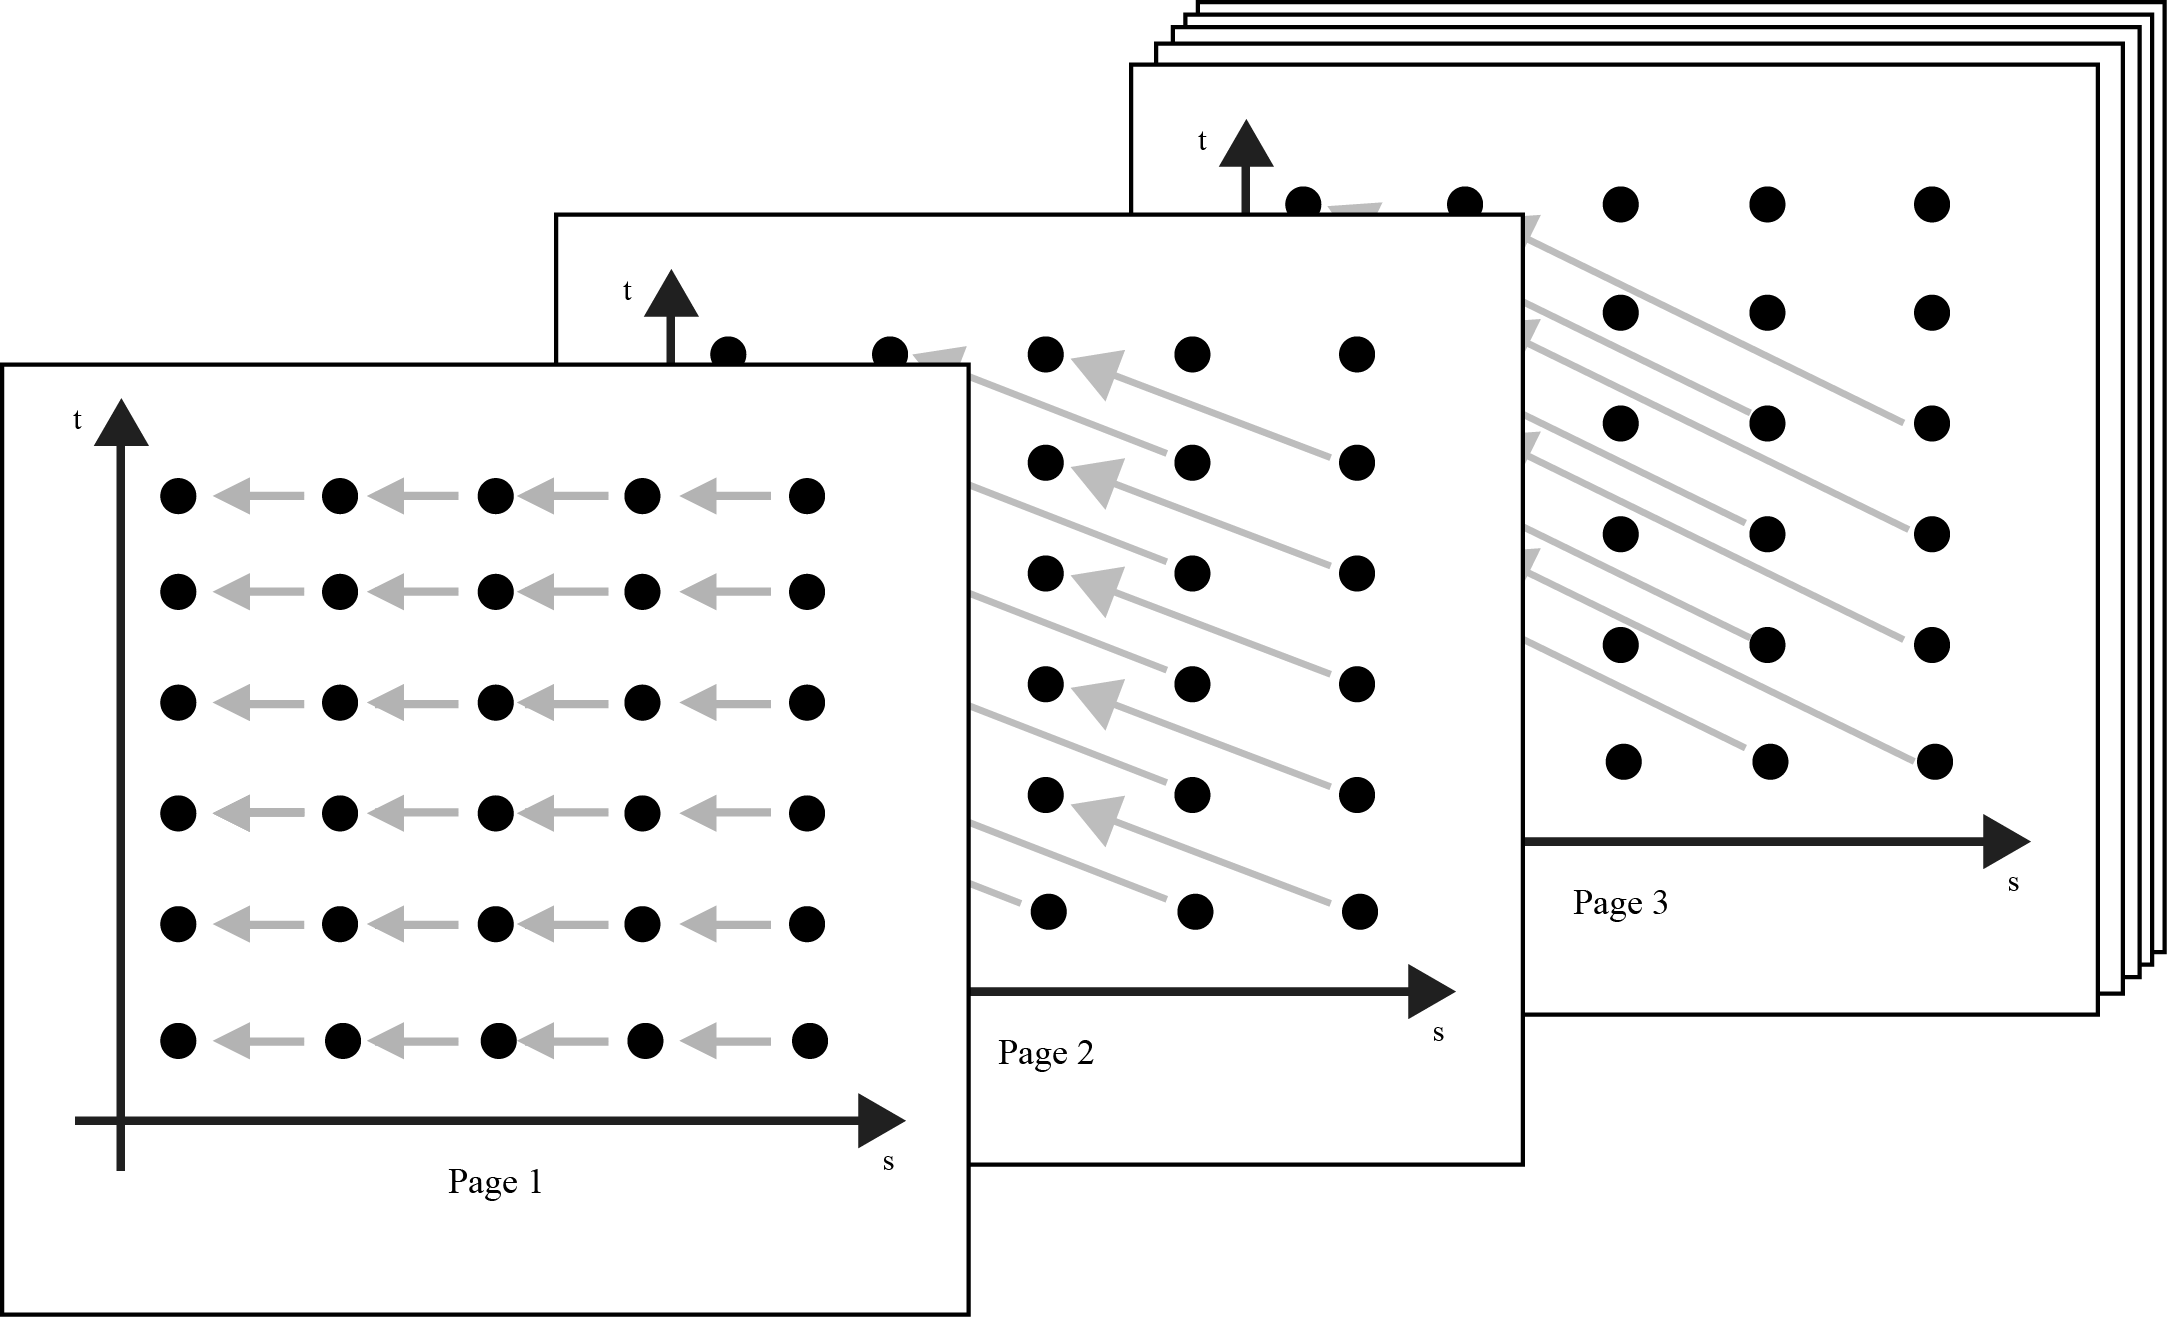
\includegraphics[width=\linewidth,height=0.5\textheight,keepaspectratio]{figures/cover.png}
  \end{center}
       \begin{minipage}{.35\linewidth}
    \begin{flushleft}
      \vspace{2em}
      {\fontsize{6pt}{2pt} \textit{Notes: These were taken during a
reading course on smooth manifolds. } } \\
    \end{flushleft}
    \end{minipage}
    \hfill
    \begin{minipage}{.65\linewidth}
    \end{minipage}
  }







\begin{document}

\date{}
\maketitle
\begin{flushleft}
\textbf{D. Zack Garza} \\
\textit{University of Georgia} \\
\textit{dzackgarza@gmail.com} \\
{\tiny \textit{Last updated:} 2020-10-25 }
\end{flushleft}


\newpage
\tableofcontents

\hypertarget{general-notes-to-self}{%
\section{General Notes to Self}\label{general-notes-to-self}}

Interesting things to know:

\begin{itemize}
\tightlist
\item
  The Whitney embedding theorem
\item
  The Jordan-Brouwer separation theorem
\item
  The Poincare-Hopf theorem
\item
  The Hopf degree theorem
\item
  Generalized Stokes' Theorem
\item
  Sard's Theorem
\item
  The Frobenius Integrability Theorem
\end{itemize}

\hypertarget{preface-point-set-review}{%
\section{Preface: Point Set Review}\label{preface-point-set-review}}

\hypertarget{quotients}{%
\subsection{Quotients}\label{quotients}}

\begin{description}
\item[Definition (Saturated)]
A subset \(A\subseteq X\) is \emph{saturated} with respect to
\(p:X\to Y\) if whenever
\(p\inv(\theset{y}) \intersect A \neq \emptyset\), then
\(p\inv(\theset{y}) \subseteq A\).

Equivalently, \(A = p\inv(B)\) for some \(B\subseteq Y\), i.e.~it is a
complete inverse image of some subset of \(Y\), i.e.~\(A\) is a union of
fibers \(p\inv(b)\).
\item[Definition (Quotient Map)]
A continuous surjective map \(p: X\surjects Y\) is a \emph{quotient map}
if \(U\subseteq Y\) is open \textbf{iff} \(p\inv(U) \subset X\) is open.

\begin{quote}
Note that \(\implies\) comes from the definition of continuity of \(p\),
but \(\impliedby\) is a stronger condition.
\end{quote}

Equivalently, \(p\) maps saturated subsets of \(X\) to open subsets of
\(Y\).
\item[Definition (Universal Property of Quotients)]
For \(\pi :X\to Y\) a quotient map, if \(g:X\to Z\) is a map that is
constant on each \(p\inv(\theset{y})\), then there is a unique map \(f\)
making the following diagram commute:

\begin{center}
\begin{tikzcd}
X \ar[d, "\pi"] \ar[rd, "g"] & \\
Y \ar[r, "f", dotted] & Z
\end{tikzcd}
\end{center}
\end{description}

Fact: an injective quotient map is a homeomorphism.

Fact: a product of quotient maps need not be a quotient map.

\hypertarget{subspaces}{%
\subsection{Subspaces}\label{subspaces}}

\begin{description}
\item[Definition (The Subspace Topology)]
\(U\subset A\) is open iff \(U = V\intersect A\) for some open
\(V\subseteq X\).
\item[Proposition (Universal Property of Subspaces)]
If \(X\) and \(\iota_S: S\injects Y\) is a subspace, then every
continuous map \(f: X\to S\) lifts to a continuous map
\(\tilde f: X\to Y\) where \(\tilde f \definedas \iota_S \circ f\):

\begin{center}
\begin{tikzcd}
 & Y \\
X \ar[r, "f"] \ar[ur, "\exists! \tilde f", dotted] & S \ar[u, "\iota_S"', hook]
\end{tikzcd}
\end{center}

Note that we can view \(\iota_S \definedas \restrictionof{\id_Y}{S}\).
The subspace topology is the unique topology for which this property
holds.
\end{description}

Some properties of subspace:

\begin{itemize}
\tightlist
\item
  The inclusion \(\iota_S\) is a topological embedding.
\item
  Restricting a continuous map to a subspace is still continuous.
\item
  A basis for the subspace topology for \(A\subset X\) can be obtained
  by intersecting basis elements of \(X\) with \(A\).
\item
  If \(X\) is Hausdorff/first/second-countable, then so is \(A\).
\end{itemize}

\hypertarget{products}{%
\subsection{Products}\label{products}}

\begin{description}
\tightlist
\item[Definition (The Product Topology)]
The coarsest topology such that every projection map
\(p_\alpha: \prod_\beta X_\beta \to X_\alpha\) is continuous, i.e.~for
every \(U_\alpha \subseteq X_\alpha\) open,
\(p_\alpha\inv(U_\alpha)\in \prod X_\beta\) is open. For finite index
sets, we can take the box topology: the collection of sets of the form
\(\prod_{i=1}^N U_i\) with each \(U_i\) open in \(X_i\) forms a basis
for the product topology on \(\prod_{i=1}^N X_i\).
\end{description}

\begin{quote}
Why these differ: in \(\RR^\infty\), the set \(S = \prod (-1, 1)\) is
open in the box topology but not the product topology, since
\(\theset{0}^\infty\) is not contained in any basic open neighborhood
contained in \(S\).
\end{quote}

Some properties of products:

\begin{itemize}
\tightlist
\item
  Projections \(\pi_i\) are continuous by definition.
\item
  A basis for the product topology can be obtained by taking the product
  of bases.
\item
  A map \(f: X \into \prod Y_i\) \emph{into} a product is continuous iff
  each component function \(F_i \definedas \pi_i \circ f: X\to Y_i\) is
  continuous.

  \begin{itemize}
  \tightlist
  \item
    I.e. if we have continuous maps \(f_i:X\to Y_i\) then the composite
    map \(F = \thevector{f_1, f_2, \cdots }\) is continuous.
  \end{itemize}
\item
  Separate continuity does not imply joint continuity: A map
  \(f: \prod X_i \to Y\) \emph{out} of a product need not be continuous
  even if (defining \(\iota_j: X_j \injects \prod X_i\)) the map
  \(f\circ \iota_j: X_j \to Y\) is continuous for all arbitrary
  inclusions \(\iota_j\).
\item
  Any map of the form \(f_{\vector{a}_j}: X_j \to \prod_{i=1}^n X_i\)
  where \(x\mapsto (a_1, \cdots, a_{j-1}, x, a_{j+1}, \cdots a_n)\) is a
  topological embedding.
\item
  If \(X_i\) are Hausdorff/first/second-countable, then so is
  \(\prod_{i=1}^n X_i\).
\end{itemize}

\hypertarget{misc}{%
\subsection{Misc}\label{misc}}

\begin{description}
\tightlist
\item[Definition (Precompact)]
A subset \(A\subseteq X\) is \emph{precompact} iff its closure
\(\cl_X(A)\) is compact in \(X\).
\item[Definition (Locally Compact]
A space \(X\) is \emph{locally compact} iff every \(x\in X\) has a
neighborhood which is contained in some compact subset of \(X\).
\end{description}

\hypertarget{analysis-review}{%
\subsection{Analysis Review}\label{analysis-review}}

\begin{description}
\item[Definition (Derivative, Real Valued)]
A function \(f:(a, b) \to \RR\) is differentiable at \(x\) iff there is
a number \(y \in \RR\) such that \begin{align*}
\qty{ {f(x+h) - f(x) \over h} - y } \converges{h\to 0}\to 0
\end{align*} where \(h\in \RR\).

The number \(f'(x) \definedas y\) is the \emph{derivative} of \(f\) at
\(x\).

Note that this equivalently says \begin{align*}
f(x+h) - f(x) = f'(x)h + r(h) \text{ where } {r(h) \over h}\converges{h\to 0}\to 0
.\end{align*}
\item[Definition (Derivative, Vector Valued)]
For \(\vector{f}: (a,b) \to \RR^n\), \(\vector \vector{f}'(x)\) is the
vector \(\vector y \in \RR^n\) such that \begin{align*}
\qty{ {\vector{f}(x+h) - \vector f(x) \over h} - \vector{y} } \converges{h\to 0}\to 0 \iff {\abs{ \vector f(x+h) - \vector f(x) - h \vector \vector y} \over \abs{h}}  \converges{h\to 0}\to 0
\end{align*} where \(h\in \RR\).

The vector \(\nabla f \definedas \vector y\) is the \emph{derivative}
(or \emph{gradient}) of \(f\) at \(\vector x\).

Note that this equivalently says \begin{align*}
\vector f(x + h) - \vector f(x) = h\nabla \vector f + \vector r(h) \quad\text{ where } {\vector r(h) \over h}\converges{h\to 0}\to \vector 0
.\end{align*}
\item[Definition (Derivative, General Case)]
A function \(\vector{f}: \RR^n \to \RR^m\) is differentiable iff there
exists a linear transformation \(\vector Y\) such that \begin{align*}
{\norm{ \vector f(\vector x+ \vector h) - \vector f(\vector x) - \vector Y \vector h}_{\RR^m} \over \norm{\vector h}_{\RR^n} }  \converges{\vector h \to \vector 0}\to 0
.\end{align*}

The matrix \(D_f(\vector x) \definedas \vector Y\) is the \emph{total
derivative} of \(f\) at \(\vector x\).

Note that this equivalently says \begin{align*}
\vector f(\vector x + \vector h) - \vector f( \vector x) = D_f \vector h + \vector r(\vector h) \quad\text{ where } { \norm{\vector r(\vector h)} \over \norm{\vector h} }\converges{\vector h\to \vector 0}\to \vector 0
.\end{align*}
\end{description}

\begin{quote}
Note that we can write
\((\nabla f)(\vector x) = \sum_{i=1}^n \dd{f}{x_i} \vector e_i\).
\end{quote}

\begin{description}
\tightlist
\item[Theorem (Chain Rule)]
If \(E\subset \RR^n\) and \(f:\RR^n \to \RR^m\) with
\(E \mapsvia{f} f(E) \mapsvia{g} g(f(E))\) with \(f\) differentiable at
\(\vector x_0\) and \(g\) differentiable at \(f(\vector x_0)\), then the
map \(F(\vector x)\definedas g(f(\vector x))\) is differentiable at
\(\vector x_0\) with derivative
\begin{align*}D_F(\vector x_0) = D_g(f(\vector x_0)) \cdot D_f(\vector x_0).\end{align*}
\item[Definition (Components of a Function)]
If \(\mcb_n \definedas \theset{\vector e_i} \subset\RR^n\) and
\(\mcb_m \definedas \theset{\vector u_i}\subset \RR^m\) are standard
bases and \(\vector f: \RR^n\to \RR^m\), then the \emph{components} of
\(\vector f\) are the functions \(f_i: \RR^n \to \RR\) defined by
\begin{align*}
\vector f(\vector x) = \sum_{i=1}^m f_i(\vector x)\vector u_i = \thevector{f_1(\vector x), \cdots, f_m(\vector x)}_{\mcb_m} 
.\end{align*}
\item[Definition (Partial Derivative)]
For \(\theset{{\vector e_j}}\) the standard orthonormal basis of
\(\RR^n\), define \begin{align*}
\dd{f_i}{x_j} = (D_j f_i)(\vector x) = \lim_{t\to 0} {f_i(\vector x + t {\vector e_j}) - f_i(\vector x) \over t}
.\end{align*}
\end{description}

\begin{quote}
Warning: \(f\) continuous and existence of all \(\dd{f_i}{x_j}\) does
not imply differentiability. If \(f\) is differentiable, however, then
\(D_f\) is the Jacobian matrix.
\end{quote}

\begin{description}
\item[Theorem (Derivative Equals Jacobian)]
If \(f\) is differentiable at \(\vector x_0\), then its derivative is an
\(m\times n\) matrix, its partial derivatives exist, and \begin{align*}
D_f(\vector x)\vector e_j &= \sum_{i=1}^m \dd{f_i}{x_j} \vector u_i \hfill \\
= \thevector{ \dd{\vector f}{x_1}, \cdots, \dd{\vector f}{x_n} }
&= 
\begin{bmatrix}
\nabla f_1 & \to \\
\nabla f_2 & \to \\
\vdots & \vdots \\
\nabla f_m & \to
\end{bmatrix}
= \thevector{ \nabla f_1^t, \cdots, \nabla f_m^t}^t
=\left[\begin{array}{ccc}
\frac{\partial f_{1}}{\partial x_{1}} & \cdots & \frac{\partial f_{1}}{\partial x_{n}} \\
\vdots & \ddots & \vdots \\
\frac{\partial f_{m}}{\partial x_{1}} & \cdots & \frac{\partial f_{m}}{\partial x_{n}}
\end{array}\right]
.\end{align*}
\item[Remark]
This implies that \begin{align*}
D_f(\vector x) \vector h = \sum_{i=1}^m \sum_{j=1}^n \dd{f_i}{x_j} h_j \vector u_i
.\end{align*}
\item[Theorem (Inverse Function Theorem)]
Suppose \(f\in C^1(\RR^n, \RR^n)\) and
\(D_f(\vector a) \in \Gl(n, \RR)\) for some \(\vector a\) and
\(\vector b = f(\vector a)\).

Then there exist \(U\ni \vector a\) and \(V\ni \vector b\) such that
\(f(U) = V\) and \(\restrictionof{f}{U}\) is bijective with inverse
\(g\in C^1(V)\).
\item[Theorem]
If \(f\in C^1(\RR^n)\) and \(D_f(\vector x)\in \Gl(n,\RR)\) for all
\(\vector x\in \RR^n\), then \(f\) is an open map (and thus
\emph{locally injective})
\item[Theorem (Implicit Function Theorem)]
Let \(A: \RR^n\cross \RR^m \to \RR^n\) and suppose
\(A_x: \RR^n\to \RR^n\) is invertible.

Then for every \(\vector k\in \RR^m\) there exists a unique
\(\vector h\in \RR^n\) such that \begin{align*}
A(\vector h, \vector k) = \vector 0 \qtext{and} \vector h = -A_x\inv A_y \vector k
.\end{align*}
\end{description}

\hypertarget{chapter-1-point-set-properties-of-topological-manifolds}{%
\section{Chapter 1: Point-Set Properties of Topological
Manifolds}\label{chapter-1-point-set-properties-of-topological-manifolds}}

Pages 1- 29.

\hypertarget{notes-part-1}{%
\subsection{Notes Part 1}\label{notes-part-1}}

\begin{description}
\item[Definition (Topological Manifold)]
A topological space \(M\) that satisfies

\begin{enumerate}
\def\labelenumi{\arabic{enumi}.}
\tightlist
\item
  \(M\) is Hausdorff, i.e.~points can be separated by open sets
\item
  \(M\) is second-countable, i.e.~has a countable basis
\item
  \(M\) is locally Euclidean, i.e.~every point has a neighborhood
  homeomorphic to an open subset \(\hat U\) of \(\RR^n\) for some fixed
  \(n\).
\end{enumerate}
\end{description}

The last property says \(p\in M \implies \exists U\) with
\(p\in U \subseteq M\), \(\hat U\subseteq \RR^n\), and a homeomorphism
\(\phi: U \to \hat U\).

\begin{quote}
Note that second countability is primarily needed for existence of
partitions of unity.
\end{quote}

\begin{description}
\tightlist
\item[Exercise]
Show that the in the last condition, \(\hat U\) can equivalently be
required to be an open ball or \(\RR^n\) itself.
\item[Theorem (Topological Invariance of Dimension)]
Two nonempty topological manifolds of different dimensions can not be
homeomorphic.
\item[Exercise]
Show that in a Hausdorff space, finite subsets are closed and limits of
convergent sequences are unique.
\item[Exercise]
Show that subspaces and finite products of Hausdorff (resp. second
countable) spaces are again Hausdorff (resp. second
countable).\label{ex:subspaces_and_products_of_hausdorff}
\end{description}

Thus any open subset of a topological manifold with the subspace
topology is again a topological manifold.

\begin{description}
\tightlist
\item[Exercise]
Give an example of a connected, locally Euclidean Hausdorff space that
is not second countable.
\item[Definition (Charts)]
A chart on \(M\) is a pair \((U, \phi)\) where \(U\subseteq M\) is open
and \(\phi: U \to \hat U\) is a homeormohpsim from \(U\) to
\(\hat U = \phi(U) \subseteq \RR^n\). If \(p\in M\) and
\(\phi(p) = 0 \in \bar U\), then the chart is said to be \emph{centered}
at \(p\). Note that any chart about \(p\) can be modified to a chart
\((\phi_1, \hat U_1)\) that is centered at \(p\) by defining
\(\phi_1(x) = x - \phi(v)\).
\end{description}

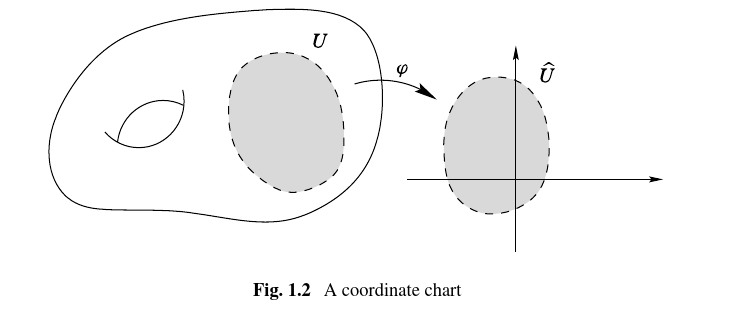
\includegraphics{figures/image_2020-06-15-00-22-05.png}

\(U\) is the \emph{coordinate domain} and \(\phi\) is the
\emph{coordinate map}.

Note that we can write \(\phi\) in components as
\(\phi(p) = \thevector{x^1(p), \cdots, x^n(p)}\) where each \(x^i\) is a
map \(x^i: U \to \RR\). The component functions \(x^i\) are the
\emph{local coordinates} on \(U\).

Shorthand notation:
\(\thevector{x^i} \definedas \thevector{x^1, \cdots, x^n}\).

\begin{description}
\item[Example (Graphs of Continuous Functions)]
Define \begin{align*}
\Gamma(f) = \theset{(x, y) \in \RR^{n} \cross \RR^{k} \suchthat x\in U,~ y = f(x) \in \hat U }
.\end{align*}

This is a topological manifold since we can take
\(\phi: \Gamma(f) \to U\) by restricting
\(\pi_1: \RR^{n}\cross \RR^k \to \RR^n\) to the subspace \(\Gamma(f)\).
Projections are continuous, restrictions of continuous functions are
continuous.\todo{Thus graphs of continuous functions $f: \RR^n \rightarrow \RR^k$ are locally Euclidean?}

This is a homeomorphism because the map \(g: x \mapsto (x, f(x))\) is
continuous and \(g\circ \pi_1 = \id_{\RR^n}\) is continuous with
\(\pi_1 \circ g = \id_{\Gamma(f)}\). Note that \(U \cong \Gamma(f)\),
and thus \((U, \phi) = (\Gamma(f), \phi)\) is a single \emph{global}
coordinate chart, called the \emph{graph coordinates} of \(f\).
\end{description}

Note that this works in greater generality::
\todo{Coordinates as numbers vs functions?} ``The same observation
applies to any subset of \(\RR^{n+k}\) by setting \emph{any} \(k\) of
the coordinates equal to some continuous function of the other \(n\).''

\begin{description}
\item[Example (Spheres)]
\(S^n\) is a subspace of \(\RR^{n+1}\) and is thus Hausdorff and
second-countable by exercise
\ref{ex:subspaces_and_products_of_hausdorff}.\label{ex:sphere_is_a_manifold}

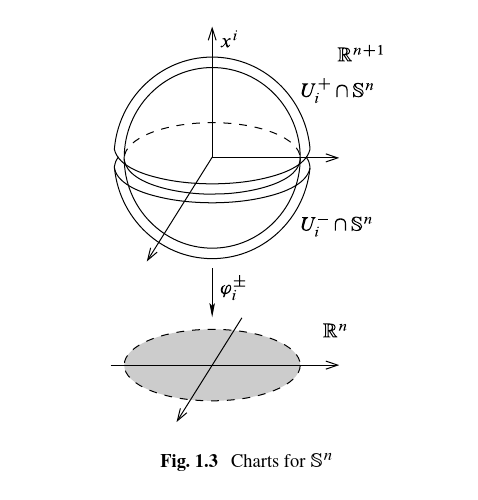
\includegraphics{figures/image_2020-06-15-21-28-56.png}

To see that it's locally Euclidean, take \begin{align*}
U_i^+ &\definedas \theset{\thevector{x^1, \cdots, x^n} \in \RR^{n+1} \suchthat x^i > 0} \qtext{for} 1 \leq i \leq n+1 \\
U_i^- &\definedas \theset{\thevector{x^1, \cdots, x^n} \in \RR^{n+1} \suchthat x^i < 0} \qtext{for} 1 \leq i \leq n+1
.\end{align*}

Define \begin{align*}
f: \RR^{n} &\to \RR^{\geq 0} \\
\vector x &\mapsto \sqrt{1 - \norm{\vector x}^2}
.\end{align*}

Note that we immediately need to restrict the domain to
\(\DD^n \subset \RR^n\), where
\(\norm{x}^2 \leq 1\implies 1 - \norm{x}^2 \geq 0\), to have a
well-defined real function \(f: \DD^n \to \RR^{\geq 0}\).

Then (claim) \begin{align*}
U_i^+ \intersect S^n \qtext{is the graph of} & x^i = f(x^1, \cdots, \hat{x^i}, \cdots, x^{n+1}) \\
U_i^- \intersect S^n \qtext{is the graph of} &x^i = -f(x^1, \cdots, \hat{x^i}, \cdots, x^{n+1})
.\end{align*}

This is because \begin{align*}
  \Gamma(x^i) 
&\definedas \theset{(\vector x, f(\vector x)) \subseteq \RR^n \cross \RR} \\
&= \theset{ \thevector{x_1, \cdots, \hat{x^i}, \cdots, x^{n+1}}, f\qty{\thevector{x_1, \cdots, \hat{x^i}, \cdots, x^{n+1} }}\subseteq \RR^n \cross \RR } \\
&= 
\theset{ \thevector{x_1, \cdots, \hat{x^i}, \cdots, x^{n+1} }, 
\qty{1 - \sum_{\substack{j=1 \\ j\neq i}}^{n+1} (x^j)^2}^{1\over 2} 
\subseteq \RR^n \cross \RR } \\
\end{align*}

and any vector in this set has norm satisfying \begin{align*}
\norm{(\vector x, y)}^2 =
\sum_{\substack{j=1 \\ j\neq i}}^{n+1} (x^j)^2 + 
\qty{1 - \sum_{\substack{j=1 \\ j\neq i}}^{n+1} (x^j)^2} = 1
\end{align*} and is thus in \(S^n\).

To see that any such point also has positive \(i\) coordinate and is
thus in \(U_i^+\), we can rearrange (?) coordinates to put the value of
\(f\) in the \(i\)th coordinate to obtain
\todo[fancyline]{Seems like $f$ is always the *last* coordinate in the graph}
\begin{align*}
\Gamma(x_i) = \theset{\thevector{x^1, \cdots, f(x^1, \cdots, \hat{x^i}, \cdots, x^n), \cdots, x^n  }}
\end{align*} and note that the square root only takes on positive
values.

Thus each \(U_i^{\pm} \intersect S^n\) is the graph of a continuous
function and thus locally Euclidean, and we can define chart maps
\begin{align*}
\phi_i^{\pm}: U_i^{\pm} \intersect S^n &\to \DD^n \\
\thevector{x^1, \cdots, x^n} &\mapsto [x^1, \cdots, \hat{x^i}, \cdots, x^{n+1}]
\end{align*} yield \(2(n+1)\) charts that are graph coordinates for
\(S^n\).
\item[Example (Projective Space)]
Define \(\RP^n\) as the space of 1-dimensional subspaces of
\(\RR^{n+1}\) with the quotient topology determined by the map
\hspace{10em} \todo[fancyline]{How is this map a quotient map?}
\begin{align*}
\pi: \RR^{n+1}\smz &\to \RP^n\\
\vector x &\mapsto \spanof_\RR\theset{\vector x}
.\end{align*}

Notation: for \(\vector x \in \RR^{n+1}\smz\) write
\([\vector x] \definedas \pi(\vector x)\), the line spanned by
\(\vector x\).

Define charts: \begin{align*}
\tilde U_i \definedas \theset{\vector x \in \RR^{n+1}\smz \suchthat x^i \neq 0}, \quad U_i = \pi(\tilde U_i) \subseteq \RP^n \\
.\end{align*}

and chart maps \begin{align*}
\tilde \phi_i: \tilde U_i &\to \RR^n \\
\thevector{x^1, \cdots, x^{n+1}} &\mapsto \thevector{{x^1 \over x^i}, \cdots \hat{x^i}, \cdots {x^{n+1} \over x^i}  }
.\end{align*}

Then (claim) this descends to a continuous map \(\phi_i: U_i \to \RR^n\)
by the universal property of the quotient:

\begin{center}
\begin{tikzcd}
\tilde U_i \ar[d, "\pi_U"'] \ar[rd, "\tilde \phi_i"] & \\
U_i \ar[r, "\phi_i", dotted] & \RR^n
\end{tikzcd}
\end{center}

\begin{itemize}
\item
  The restriction \(\pi_U: \tilde U_i \to U_i\) of \(\pi\) is still a
  quotient map because \(\tilde U_i = \pi_U\inv(U_i)\) where
  \(U_i\subseteq \RP^n\) is open in the quotient topology and thus
  \(\tilde U_i\) is saturated.

  Thus \(\pi_U\) sends saturated sets to open sets and is thus a
  quotient map.
\item
  \(\tilde \phi_i\) is constant on preimages under \(\pi_U\): fix
  \(y\in U_i\), then
  \(\pi_U\inv(\theset{y}) = \theset{\lambda \vector y \suchthat \lambda \in \RR\smz}\),
  i.e.~the point \(y \in \RP^n\) pulls back to every nonzero point on
  the line spanned by \(\vector y\in \RR^n\).

  But \begin{align*}
  \tilde \phi_i(\lambda \vector y) 
  &= \phi_i \qty{ \thevector{\lambda y^1, \cdots, \lambda y^i, \cdots, \lambda y^n} } \\
  &= \thevector{{\lambda y^1 \over \lambda y^i}, \cdots, \hat{\lambda y^i}, \cdots, {\lambda y^{n+1} \over \lambda y^i}} \\
  &= \thevector{{y^1 \over y^i}, \cdots, \hat{y^i}, \cdots, {y^{n+1} \over y^i}} \\
  &= \tilde \phi_i(\vector y)
  .\end{align*}
\end{itemize}
\end{description}

So this yields a continuous map \begin{align*}
  \phi_i: U_i \to \RR^n
  .\end{align*}

We can now verify that \(\phi\) is a homeomorphism since it has a
continuous inverse given by

\begin{align*}
  \phi_i\inv: \RR^n &\to U_i \subseteq \RP^n \\
  \vector u \definedas \thevector{u^1, \cdots, u^n } &\mapsto \thevector{u^1, \cdots, u^{i-1}, {\color{red}1}, u^{i+1}, \cdots, u^n}
  .\end{align*}

It remains to check: \todo{Exercise}

\begin{enumerate}
\def\labelenumi{\arabic{enumi}.}
\tightlist
\item
  The \(n+1\) sets \(U_1, \cdots, U_{n+1}\) cover \(\RP^n\).
\item
  \(\RP^n\) is Hausdorff
\item
  \(\RP^n\) is second-countable.
\end{enumerate}

\begin{description}
\item[Exercise (1.6)]
Show that \(\RP^n\) is Hausdorff and second countable.
\item[Exercise (1.7)]
Show that \(\RP^n\) is compact. (Hint: show that \(\pi\) restricted to
\(S^n\) is surjective.)
\item[Definition (Topological Embedding)]
A continuous map \(f:X\to Y\) is a \emph{topological embedding} iff it
is injective and \(\tilde f:X\to f(X)\) is a homeomorphism.
\item[Example (Product Manifolds)]
Let \(M \definedas M_1 \times \cdots \times M_k\) be a product of
manifolds of dimensions \(n_1, \cdots, n_k\) respectively. A product of
Hausdorff/second-countable spaces is still Hausdorff/second-countable,
so just need to check that it's locally Euclidean.

\begin{itemize}
\item
  Let \(\vector p \in \prod_{i=1}^N M_i\), so \(p_i \in M_i\)
\item
  Choose a chart \((U_i, \phi_i)\) with \(p_i\in U_i\) and assymble a
  product map: \begin{align*}
  \Phi \definedas \prod \phi_i: \prod U_i \to \prod R^{n_i} \cong \RR^{\Sigma n_i} \definedas \RR^N
  .\end{align*}
\item
  Claim: \(\Phi\) is a homeomorphism onto its image in \(R^N\).

  \begin{itemize}
  \tightlist
  \item
    Each \(\phi_i\) is a homeomorphism onto \(\phi_i(U_i)\) (by the
    definition of a chart on \(M_i\))
  \item
    It suffices to show that that \(\Phi\inv\) exists and is continuous,
    where \begin{align*}
    \Phi\inv(V) \definedas \qty{\prod \phi_i}\inv \qty{\prod V_i}
    .\end{align*}
  \item
    \(\Phi\) is a product of continuous functions and thus continuous.
  \item
    \(\Phi\inv \definedas \qty{\prod \phi_i}\inv = \prod \phi_i\inv\),
    which are all assumed continuous since \(\phi_i\) were
    homeomorphisms.
  \end{itemize}
\end{itemize}
\item[Example (Torii)]
\(T^n \definedas \prod_{i=1}^n S^1\) is a topological
\(n\dash\)manifold.
\item[Definition (Precompact)]
A subset \(A\subseteq X\) is \emph{precompact} iff its closure
\(\cl_X(A)\) is compact in \(X\).
\item[Proposition]
Every topological manifold has a countable basis of precompact
coordinate balls.
\item[Proposition]
Let \(M\) be a topological manifold.

\begin{itemize}
\tightlist
\item
  \(M\) is locally path-connected.
\item
  \(M\) is connected \(\iff M\) is path-connected
\item
  The connected components and path components of \(M\) coincide.
\item
  \(\pi_0(M)\) is countable and each component is open and a connected
  topological manifold.
\end{itemize}
\item[Proposition]
Every topological manifold \(M\) is locally compact.
\item[Proof]
\(M\) has a basis of precompact open sets.
\item[Theorem (Manifolds are Paracompact)]
Given any open cover \(\mcu \covers M\) of a topological manifold and
any basis \(\mcb\) for the topology on \(M\), there exists a countable
locally finite open refinement of \(\mcu\) consisting of elements of
\(\mcb\).
\item[Proposition]
\(\pi_1(M)\) is countable.
\end{description}

\hypertarget{notes-part-2}{%
\subsection{Notes Part 2}\label{notes-part-2}}

\begin{description}
\item[Definition (Smooth Functions)]
A function \(f:\RR^n \to \RR^m\) given by
\(\thevector{f_1(\vector x^n), f_2(\vector x^n), \cdots, f_m(\vector x^n)}\)
(or any subsets thereof) is said to be \(C^\infty\) or \textbf{smooth}
iff each \(f_i\) has continuous partial derivatives of all orders.
\item[Definition (Diffeomorphism)]
A smooth bijective map with a smooth inverse is a \emph{diffeomorphism}.
\item[Remark]
A diffeomorphism is necessarily a homeomorphism, but not conversely.
\item[Definition (Transition Maps)]
If \((U, \phi), (V, \psi)\) are two charts on \(M\) such that
\(U\intersect V \neq \emptyset\), the composite map
\(\psi \circ \phi\inv: \phi(U\intersect V) \to \psi(U\intersect V)\) is
a function \(\RR^n\to\RR^n\) and is called the \emph{transition map}
from \(\phi\) to \(\psi\).
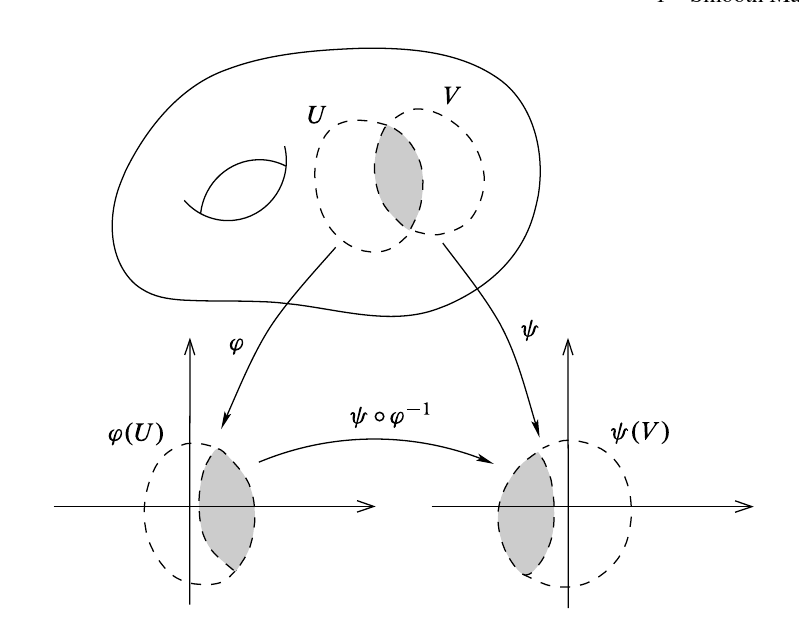
\includegraphics{figures/image_2020-06-21-22-39-09.png} Two charts are
\emph{smoothly compatible} iff \(U\intersect V = \emptyset\) or
\(\psi \circ \phi\inv\) is a diffeomorphism.
\item[Definition]
A collection of charts
\(\mca \definedas \theset{(U_\alpha, \phi_\alpha)}\) is an \emph{atlas}
for \(M\) iff \(\theset{U_\alpha} \covers M\), and is a \emph{smooth
atlas} iff all of the charts it contains are pairwise smoothly
compatible.
\item[Remark]
To show an atlas is smooth, it suffices to show that an arbitrary
\(\psi \circ \phi\inv\) is smooth. This is because this immediately
implies that its inverse is smooth, and these these are diffeomorphisms.
Alternatively, one can show that \(\psi\circ\phi\inv\) is smooth,
injective, and has nonsingular Jacobian at each point.
\item[Remark]
Attempting to define a function \(f: M\to \RR\) to be smooth iff
\(f\circ \phi\inv: \RR^n \to \RR\) is smooth for each \(\phi\) may not
work because many atlases give the ``same'' smooth structure in the
sense that they all determine the same collection of smooth functions on
\(M\).
\todo{What does "determine the same collection of smooth functions" mean?}

For example, take the following two atlases on \(\RR^n\): \begin{align*}
\begin{array}{l}
{\mca}_{1}=\left\{\left(\mathbb{R}^{n}, \operatorname{Id}_{\mathbb{R}^{n}}\right)\right\} \\
{\mca}_{2}=\left\{\left(\DD_{1}(\vector x), \id_{\DD_{1}(\vector x)}\right)\suchthat \vector x \in \mathbb{R}^{n}\right\}
\end{array}
.\end{align*}

Claim: a function \(f:\RR^n \to \RR\) is smooth wrt either atlas iff it
is smooth in the usual sense.
\item[Definition (Maximal or Complete Atlas)]
A smooth atlas on \(M\) is \emph{maximal} iff it is not properly
contained in any larger smooth atlas.
\item[Remark]
Not every topological manifold admits a smooth structure. See Kervaire's
10-dimensional manifold from 1960.
\item[Definition (Smooth Structures and Smooth Manifolds)]
If \(M\) is a topological manifold, a maximal smooth atlas \(\mca\) is a
\emph{smooth structure} on \(M\). The triple \((M, \tau, \mca)\) where
\(\mca\) is a smooth structure is a \emph{smooth manifold}.
\item[Remark]
To show that two smooth structures are \emph{distinct}, it suffices to
show that they are not smoothly compatible, i.e.~one of the transition
functions \(\psi\circ \phi\inv\) is not smooth. This is because any
maximal atlas \(\mca_1\) must contain \(\psi\) and likewise \(\mca_2\)
contains \(\phi\inv\), but no maximal atlas can contain \(\phi\)
\emph{and} \(\psi\) because all charts in a maximal atlas are smoothly
compatible by definition.
\item[Proposition]
Let \(M\) be a topological manifold.

\begin{enumerate}
\def\labelenumi{\arabic{enumi}.}
\tightlist
\item
  Every smooth atlas \(\mca\) for \(M\) is contained in a unique maximal
  smooth atlas, called the \emph{smooth structure determined by
  \(\mca\)}.
\item
  Two smooth atlases for \(M\) determine the same smooth structure
  \(\iff\) their union is a smooth atlas.
\end{enumerate}
\item[Remark]
That we can place many requirements on the functions
\(\psi \circ \phi\inv\) and get various other structures: \(C^k\),
real-analytic, complex-analytic, etc. \(C^0\) structures recover
topological manifolds.
\item[Definition (Smooth Charts, Maps, Domains)]
If \((M,\ \tau, \mca)\) is a smooth manifold, any chart
\((U, \phi)\in \mca\) is a \emph{smooth chart}, where \(U\) is a
\emph{smooth coordinate domain} and \(\phi\) is a \emph{smooth
coordinate map}. A \emph{smooth coordinate ball} is a smooth coordinate
domain \(U\) such that \(\phi(U) = \DD^n\).
\item[Definition (Regular Coordinate Ball)]
A set \(B\subseteq M\) is a \emph{regular coordinate ball} if there is a
smooth coordinate ball \(B'\) such that \(\cl_M(B) \subseteq B'\), and a
smooth coordinate map \(\phi: B'\to \RR^n\) such that for some positive
numbers \(r < r'\),

\begin{itemize}
\tightlist
\item
  \(\phi(B) = \DD_r(\vector 0)\),
\item
  \(\phi(B') = \DD_{r'}(\vector 0)\), and
\item
  \(\phi(\cl_M(B)) = \cl_{\RR^n}(\DD_r(\vector 0))\).
\end{itemize}

This says \(B\) ``sits nicely'' insane a larger coordinate ball.
\item[Remark]
\(\cl_M(B) \cong_{\Top} \cl_{\RR^n}(\DD_r(\vector 0))\) which is closed
and bounded and thus compact, so \(\cl_M(B)\) is compact. Thus every
regular coordinate ball in \(M\) is precompact.
\item[Proposition]
Every smooth manifold has a countable basis of regular coordinate balls.
\item[Remark]
There is only one 0-dimensional smooth manifold, up to equivalence of
smooth structures.
\item[Definition (Standard Smooth Structure on
\$\textbackslash RR\^{}n\$)]
Define the atlas \(\mca_0 = \theset{(\RR^n, \id_{\RR^n})}\) and take the
smooth structure it generates, this is the \emph{standard smooth
structure} on \(\RR^n\).
\item[Proposition]
There are at least two distinct smooth structures on \(\RR^n\).
\item[Proof]
Define \(\psi(x) = x^3\); then
\(\mca_1 \definedas \theset{(\RR^n, \phi)}\) defines a smooth structure.

Then \(\mca_1 \neq \mca_0\), which follows because
\(\qty{\id_{\RR^n} \circ \phi\inv}(x) = x^{1\over 3}\), which is not
smooth at \(\vector 0\).
\end{description}

\hypertarget{recommended-problems}{%
\subsection{Recommended Problems}\label{recommended-problems}}

\begin{quote}
Note: helpful theorem, two smooth structures induced by two smooth
atlases \(\mca_1, \mca_2\) are equivalent iff \(\mca_1 \union \mca_2\)
is again a smooth atlas. So it suffices to check pairwise compatibility
of charts.
\end{quote}

\begin{description}
\item[Exercise (Problem 1.6)]
Show that if \(M^n\neq \emptyset\) is a topological manifold of
dimension \(n\geq 1\) and \(M\) has a smooth structure, then it has
uncountably many distinct ones. \todo{Recommended problem}

\begin{quote}
Hint: show that for any \(s> 0\) that
\(F_s(x) \definedas \abs{x}^{s-1}x\) defines a homeomorphism
\(F_x: \DD^n \to \DD^n\) which is a diffeomorphism iff \(s=1\).
\end{quote}
\end{description}

Solution:

Define \begin{align*}
F_s: \RR^n &\to \RR^n \\
\vector x &\mapsto \norm{\vector x}^{s-1} \vector x 
.\end{align*}

Claim: \(F_s\) restricted to \(\DD^n\) is a continuous map
\(\DD^n \to \DD^n\).

\begin{itemize}
\item
  Note that if \(\norm{\vector x}\leq \eps < 1\) then
  \begin{align*}\norm{F_s(\vector x)} = \norm{ \norm{\vector x}^s \hat{\vector x} } = \norm{\vector x}^s \leq \norm{\vector x} \leq \eps < 1,\end{align*}
  so \(F_s(\DD^n) \subseteq \DD^n\) and moreover
  \(F_s(\DD_\eps^n) \subseteq \DD_\eps^n\).

  \begin{itemize}
  \tightlist
  \item
    We'll use the fact that \(F_s\inv = F_{1\over s}\) is of the same
    form, and thus \(F_s\inv(\DD^n) \subseteq \DD^n\), forcing
    \(F_s(\DD^n) = \DD^n\).
  \end{itemize}
\item
  This is a continuous function on the punctured disc
  \(\DD_0^n \definedas \DD^n\setminus\theset{\vector 0}\), since it can
  be written as a composition of smooth functions:

  \begin{center}
   \begin{tikzcd}
  \DD_0^n \ar[r, "\Delta"] & \DD_0^n \cross \DD_0^n \ar[r, "{(\norm{\wait}, ~\id_{\DD_0^n})}", outer sep=5pt] & \DD_0^n \cross \DD_0^n \ar[r, "{(\qty{\wait }^{s-1}, ~\id_{\DD_0^n})}", outer sep=5pt] & \DD_0^1 \cross \DD_0^n \ar[r, "{(a,b)\mapsto ab}", outer sep=5pt]& \DD_0^n \\
    \vector x \ar[r] & (\vector x, \vector x) \ar[r] & (\norm{\vector x}, \vector x) \ar[r] & (\norm{\vector x}^{s-1}, \vector x)\ar[r] & \norm{\vector x}^{s-1} \vector x
   \end{tikzcd}
   \end{center}

  For any \(s\geq 0\), continuity at zero follows from the fact that
  \(\norm{F_s(\vector x)} \leq \norm{\vector x} \to 0\), so
  \(\lim_{\vector x \to \vector 0}F_s(\vector x) = \vector 0\) and the
  sequential definition of continuity applies. So \(F_s\) is continuous
  on \(\DD^n\) for every \(s\).

  \begin{quote}
  Here we are taking for granted the fact that taking norms,
  exponentiating, and multiplying are all smooth functions away from
  zero.
  \end{quote}
\end{itemize}

Claim: \(F_s\) is a bijection \(\DD^n\setminus{\vector 0}\selfmap\) that
extends to a bijection \(\DD^n\selfmap\).

We can note that \begin{align*}
F_s(\vector x) = 
\begin{dcases}
\norm{\vector x}^s{\vector x \over \norm{\vector x}} \definedas \norm{\vector x}^s \hat{\vector x} & \text{if } \norm{\vector x} \neq 0 \\
\vector 0 & \text{if } \norm{\vector x } = 0
\end{dcases}
\end{align*}

This follows because we can construct a two-sided inverse that composes
to the identity, namely \(F_{1\over s}\), for
\(\vector x\neq \vector 0\), and note that
\(F_s(\vector 0) = \vector 0\). Using the fact that
\(\norm{t \vector x} = t\norm{\vector x}\) for any scalar \(t\), we can
check that \begin{align*}
\qty{F_s \circ F_{1\over s}}(\vector x)
&= F_s(\norm{\vector x}^{1\over s} \hat{\vector x}) \\
&= \norm{ \norm{\vector x}^{1\over s} \hat{\vector x} }^{s} \cdot \hat{\norm{\vector x}^{1\over s} \hat{\vector x}} \\
&= \qty{ \norm{\vector x}^{1\over s}}^s \cdot \norm{ \hat{\vector x} }^{s} \cdot { \norm{\vector x}^{1\over s} \hat{\vector x} \over \norm{ \norm{\vector x}^{1\over s} \hat{\vector x}  } } \\
&= \norm{\vector x} \cdot 1^s \cdot \qty{\norm{\vector x}^{1\over s} \over \norm{\vector x}^{1\over s}} \cdot {\hat{\vector x} \over \norm{\hat{\vector x}} } \\
&= \norm{\vector x} \hat{\vector x} \\
&= \vector x
.\end{align*}

and similarly \begin{align*}
\qty{F_{1\over s} \circ F_s}(\vector x) 
&= F_{1\over s} \qty{ \norm{\vector x}^s \hat{\vector x}  } \\
&= \norm{\norm{\vector x}^s \hat{\vector x}  }^{1\over s} \cdot \hat{ \norm{\vector x}^s \hat{\vector x}  } \\
&= \qty{\norm{\vector x}^s}^{1\over s} \norm{\hat{\vector x} }^{1\over s} \cdot {\norm{\vector x}^s \hat{\vector x} \over \norm{ \norm{\vector x}^s \hat{\vector x} }  } \\
&= \norm{\vector x} \cdot 1^{1-s} \cdot \qty{\norm{\vector x}^s \over \norm{\vector x}^s } \cdot {\hat{\vector x} \over \norm{\hat{\vector x}}} \\
&= \norm{\vector x} \hat{\vector x} \\
&= \vector x
.\end{align*}

Claim: \(F_s\) is a homeomorphism for all \(s\).

This follows from the fact that the domain \(\DD^n\) is compact and the
codomain \(\DD^n\) is Hausdorff, and a continuous bijection between such
spaces is a homeomorphism.

Claim: \(F_s\) is a diffeomorphism iff \(s=1\).

If \(s=1\), \(F_s = \id_{\DD^n}\) which is clearly a diffeomorphism.

Otherwise, we claim that \(F_s\) is not a diffeomorphism because either
\(F_s\) or \(F_s\inv\) will fail to be smooth at
\(\vector x = \vector 0\).

\begin{itemize}
\tightlist
\item
  If \(0\leq s < 1\), then \(F_s\) fails to be differentiable at zero.
  \todo{Why? Should boil down to $x\mapsto x^t$ for $0\leq t< 1$ failing to be differentiable at 0 in $\RR$}
\item
  If \(1<s< \infty\) then \(0 \leq {1\over s} < 1\) and the same
  argument applies to \(F_s\inv \definedas F_{1\over s}\).
\end{itemize}

We now show that we can produce infinitely many distinct maximal atlases
on \(M\). Let \(\mca\) by any smooth atlas on \(M\) and fix
\(p_0\in M\).

Claim: We can modify \(\mca\) to obtain an atlas \(\mca'\) where \(p_0\)
is in exactly one chart \((V, \psi)\) with
\(\psi(p_0) = \vector 0 \in \RR^n\).

\begin{itemize}
\tightlist
\item
  Pick a chart containing \(p_0\), say \((U, \phi)\) where
  \(\phi(p_0) \definedas \vector p\)
\item
  Since \(\phi(U)\subseteq \RR^n\) is open, find a disc containing
  \(\vector p\), say \(\DD_R(\vector p) \subset \phi(U)\).
\item
  Define \(V\subseteq M\) as \(V\definedas \phi\inv(\DD_R(\vector p))\).
\item
  Define \(\psi: U\to \RR^n\) by \begin{align*}
  \psi: U &\to \RR^n \\
  x &\mapsto {\phi(x) - \phi(p_0) \over R}
  .\end{align*}

  \begin{itemize}
  \tightlist
  \item
    Note: this is constructed precisely so that
    \(\psi(V) = \DD_1(\vector 0) \in \RR^n\) and \(\psi(p) = 0\).
  \item
    This is a homeomorphism onto its image since we can write
    \begin{align*}\psi = \delta_{1\over R}\circ \tau_{\vector p} \circ \phi\end{align*}
    is a composition of continuous functions, where \(\delta, \tau\) are
    dilations/translations in \(\RR^n\) which are known to be
    continuous, and
    \begin{align*}\psi\inv = \phi\inv \circ \tau_{- \vector p} \circ \delta_R\end{align*}
    is again a composition of smooth (and in particular, continuous)
    functions.
  \end{itemize}
\item
  Define
  \(\mca^1 \definedas \mca \union \theset{ (V, \restrictionof{\psi}{V})}\)

  \begin{itemize}
  \tightlist
  \item
    This is a smooth atlas: any pair of charts coming from \(\mca\) are
    smoothly compatible, so it suffices to check that an arbitrary chart
    from \(\mca\) is smoothly compatible with the new chart.
  \item
    Let \((T, \xi)\) be any other chart, then if
    \(T\intersect V\neq \emptyset\), the transition function
    \begin{align*}\psi \circ \xi\inv =  \delta_{1\over R} \tau_{\vector p} \circ \phi \circ \xi\inv\end{align*}
    is a composition of smooth functions and thus smooth, and similarly
    for \(\xi\circ \psi\inv\).
  \item
    Since the charts from \(\mca\) cover \(M\), so do the charts of
    \(\mca^1\) since \(\mca \subseteq \mca^1\).
  \end{itemize}
\item
  For every \((U_\alpha, \phi_\alpha)\in \mca^1\), define a new chart
  \((U_\alpha \setminus\theset p, \restrictionof{\phi_\alpha}{U_\alpha \setminus\theset p})\)
  and define this set of charts as \(\mca^2\).

  \begin{itemize}
  \tightlist
  \item
    This still covers \(M\): \(p\) is in the chart \((V, \psi\mid_V)\),
    and if \(q\neq p\), then \(q\in U_\alpha\) for some \(\alpha\) since
    \(\mca\) was an atlas, and \(q\in U_\alpha\setminus\theset{p}\).
  \item
    The coordinate maps are still homeomorphisms onto their images,
    because the restriction of a homeomorphism is again a homeomorphism.
  \item
    The transition functions are still smooth because the restriction of
    a smooth function is again smooth.
  \end{itemize}
\end{itemize}

Claim: We can define a new atlas \(\mca_s\) from \(\mca^2\) by only
replacing the single chart \((V, \psi)\) with \((V, F_s \circ \psi)\).

\begin{itemize}
\tightlist
\item
  \(\mca_s\) still covers \(M\), since we haven't changed the coordinate
  domains
\item
  All coordinate functions are still a homeomorphisms onto their images,
  since the only change is \(\psi\) is replaced with \(F_s \circ \psi\)
  and we've shown that \(F_s\) is a homeomorphism; a composition of
  homeomorphisms is again a homeomorphism.
\item
  The chart \((V, F_s\circ \psi)\) is still a valid chart, since
  \(F_s: \DD_n\selfmap\) and \(\psi(V) \cong \DD^n\) by construction.
\item
  All charts in \(\mca_s\) are still smoothly compatible:

  \begin{itemize}
  \tightlist
  \item
    If suffices to check compatibility between an arbitrary
    \((U_\alpha, \phi_\alpha)\) and \((V, F_s\circ \psi)\), so we
    consider \(F_s\circ \psi\circ \phi_\alpha\inv\)
  \item
    By construction, \(p\not\in U_\alpha\), and we know \(F_s\) is
    smooth away from \(\vector 0\), so this is a smooth function.
  \end{itemize}
\end{itemize}

Claim: If \(s\neq t\) then \(\mca_s\) and \(\mca_t\) are not smoothly
compatible, and thus generate distinct maximal smooth atlases.

\begin{itemize}
\tightlist
\item
  If \(\mca_s, \mca_t\) define the same smooth structure, then in
  particular \((V, F_s\circ \psi)\) must be smoothly compatible with
  \((V, F_t \circ \psi)\).
\item
  We can compute the transition function \begin{align*}
  \qty{F_s\circ \psi} \circ (F_t\circ \psi)\inv = F_s\circ \psi \circ \psi\inv \circ F_t\inv = F_s\circ F_t\inv = F_s \circ F_{1\over t} = F_{s\over t}
  .\end{align*}
\item
  From above, we know this is smooth iff \({s\over t} = 1\),
  i.e.~\(s=t\).
\item
  So if \(s\neq t\), then the maximal atlases correspond to
  \(\mca_s, \mca_t\) each contain a chart that is not smoothly
  compatible with the other, and so these are distinct smooth
  structures.
\end{itemize}

\(\qed\)

\begin{description}
\item[Exercise (Problem 1.7)]
Let \(N\definedas \thevector{0, \cdots, 1} \in S^n\) and
\(S\definedas \thevector{0, \cdots, -1}\) and define the stereographic
projection \todo{Recommended problem} \begin{align*}
\sigma: S^n\setminus N &\to \RR^n \\
\thevector{x^1, \cdots, x^{n+1}} &\mapsto {1 \over 1-x^{n+1}} \thevector{x^1, \cdots, x^n}
\end{align*} and set \(\tilde\sigma(x) = -\sigma(-x)\) for
\(x\in S^n\setminus S\) (projection from the South pole)
\todo{Note that the figure should say $\theset{x^{n+1} = 0}$ instead of $x^n$.}

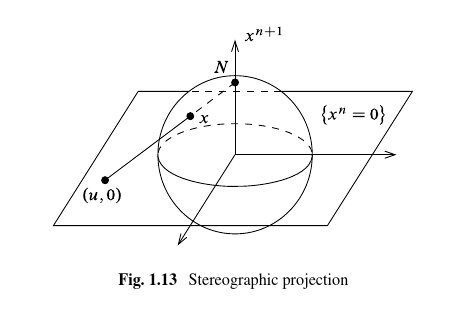
\includegraphics{figures/image_2020-06-15-23-36-33.png}

\begin{enumerate}
\def\labelenumi{\arabic{enumi}.}
\item
  For any \(x\in S^n\setminus N\) show that \(\sigma(x) = \vector u\)
  where \((\vector u, 0)\) is the point where the line through \(N\) and
  \(x\) intersects the linear subspace
  \(H_{n+1} \definedas \theset{x^{n+1} = 0}\).

  Similarly show that \(\tilde \sigma(x)\) is the point where the line
  through \(S\) and \(x\) intersects \(H_{n+1}\).
\item
  Show that \(\sigma\) is bijective and \begin{align*}
  \sigma\inv(\vector u) = \sigma\inv\qty{\thevector{u^1, \cdots, u^n }} = {1\over \norm{\vector u}^2 + 1} \thevector{2u^1, \cdots, 2u^n, \norm{\vector u}^2 - 1}
  .\end{align*}
\item
  Compute the transition map \(\tilde \sigma \circ \sigma\inv\) and
  verify that the atlas \begin{align*}
  \mca \definedas \theset{(S^n\setminus N, \sigma), (S^n\setminus S, \tilde \sigma)  }
  \end{align*} define a smooth structure on \(S^n\).
\item
  Show that this smooth structure is equivalent to the standard smooth
  structure: Put graph coordinates on \(S^n\) as outlined in
  \ref{ex:sphere_is_a_manifold} to obtain
  \(\theset{(U_i^\pm, \phi_i^{\pm})}\).

  For indices \(i<j\), show that \begin{align*}
   \phi_i^\pm \circ (\phi_j^\pm)\inv \thevector{u^1, \cdots, u^n} = \thevector{u^1, \cdots, \hat{u^i}, \cdots, \pm\sqrt{1 - \norm{\vector u}^2}  ,\cdots u^n}
   \end{align*} where the square root appears in the \(j\)th position.
  Find a similar formula for \(i>j\). Show that if \(i=j\), then
  \begin{align*}
   \phi_i^\pm \circ (\phi_j^\pm)\inv = \phi_i^- \circ (\phi_i^+)\inv = \id_{\DD^n} 
   .\end{align*}

  Show that these yield a smooth atlas.
\end{enumerate}
\end{description}

Solution (1):

\begin{itemize}
\item
  Parameterize the line through \(\vector x\in S^n\) and \(\vector N\):
  \begin{align*}
  \ell_{N, \vector x}(t) 
  &= t\vector x + (1-t) \vector N \\
  &= t\thevector{x^1, \cdots, x^n, x^{n+1}} + (1-t)\thevector{0, \cdots, 1} \\
  &= \thevector{tx^1, \cdots, x^n, tx^{n+1} + (1-t)} \\
  &= \thevector{tx^1, \cdots, x^n, 1 - t\qty{1-x^{n+1}}} \\
   .\end{align*}
\item
  Evaluate at \(t = {1 \over 1 - x^{n+1}}\) to obtain
  \({1\over x^{n+1}}\thevector{x^1, \cdots, x^n, 0} = \thevector{ \sigma(\vector x), 0}\).
\item
  For \(\tilde \sigma(\vector x)\): Todo \todo{Todo}.
\end{itemize}

Solution (2):

\begin{itemize}
\tightlist
\item
  How to derive this formula: no clue. \todo{Figure out how to invert.}

  \begin{itemize}
  \tightlist
  \item
    Start with \(\vector u \in \RR^n\), parameterize the line
    \(\ell_{N, \vector u}(t)\), solve for where
    \(\norm{\ell_{N, \vector u}(t)} = 1\) and \(\vector u \neq N\)
  \item
    Should yield \(t^2 \norm{u} + (1-t)^2 = 1\), solve for nonzero
    \(t\); should get \(t = {2 \over \norm{\vector u} + 1}\), so
    \(x^i = 2u^i/(\norm{\vector u} + 1)\) and
    \(x^{n+1} = \qty{2 \over \norm{\vector u} + 1} -1\).
  \end{itemize}
\item
  Compute compositions \(\sigma \circ \sigma\inv\): Todo.
  \todo{Messy computations that didn't work out.}
\end{itemize}

Solution (3):

\begin{itemize}
\item
  Computing the transition maps: \begin{align*}
  (\tilde \sigma \circ \sigma\inv)(\vector u) 
  &= -\sigma\qty{\qty{-1 \over \norm{\vector u}^2 + 1} \thevector{2u^1, \cdots, 2u^n, \norm{\vector u}^2 - 1}  } \\
  &= -1 \cdot \thevector{ {{ -2 u^1 \over \norm{\vector u}^2 + 1} \over 1 - {1 - \norm{\vector u}^2 \over 1 + \norm{\vector u}^2 }}  , \cdots_n } \\
  &= \thevector{ {2u^1 \over \norm{\vector u}^2 + 1} \cdot {1 + \norm{\vector u}^2 \over 1 + \norm{\vector u}^2 - (1 - \norm{\vector u}^2)}, \cdots_n} \\
  &= \thevector{ {2u^1 \over 2\norm{\vector u}^2}, \cdots_n } \\
  &= {\vector u \over \norm{\vector u}^2} \\
  &\definedas \hat{\vector u}
  ,\end{align*} which is a smooth function on
  \(\RR^n\setminus\theset{\vector 0}\).
\item
  Todo: computing
  \((\sigma \circ \tilde\sigma\inv)(\vector u) = \hat{\vector u}\)\todo{Computation.}
\item
  Todo: argue that it suffices that these are smooth on
  \(\RR^n\setminus\theset{\vector 0}\)
  \todo{What are the actual domains and ranges of the transition functions? It seems like you pull back $\RR^n$ to $S^n\setminus N$, then push $S^n\setminus\theset{N, S}$ to $R^n\setminus 0$, but this yields $\RR^n\to\RR^{n}\setminus 0$ where we haven't deleted zero in the domain (problem: not smooth!).}
\end{itemize}

Solution (4):

We want to argue that these define the same maximal smooth atlas, for
which it suffices to the charts from each are pairwise smoothly
compatible.

\begin{itemize}
\tightlist
\item
  Define
  \(\phi_i\qty{\thevector{x^1, \cdots, x^n}} = \thevector{x^1, \cdots, \hat{x^i}, \cdots, x^n}\)
  and
  \(\phi_i\inv\qty{\thevector{x^1, \cdots, x^{n-1}}} = \thevector{x^1, \cdots_i, \sqrt{1 - \norm{\vector x}}, \cdots, x^n }\).
\item
  Compute
  \((\phi_i \circ \sigma\inv)(\vector u) = {1 \over \norm{\vector u} + 1}\thevector{2 u^1, \cdots \hat{u^i}, \cdots, 2u^n, \norm{\vector u}^2 - 1}\),
  which is (clearly) smooth?
\item
  Compute
  \((\sigma \circ \phi_i\inv)(\vector u) = \sigma\qty{\thevector{u^1, \cdots_i, \sqrt{1 - \norm{\vector u}^2}, \cdots, u^n } }\),
  which is
  \({1\over 1-u^n}\thevector{u^1, \cdots_i, \sqrt{1-\norm{\vector u}^2}, \cdots, u^{n-1}}\).

  \begin{itemize}
  \tightlist
  \item
    This is smooth if \(u^n\neq 1\), but this corresponds to
    \(\vector N\) in \(S^2\), in which case \(\phi_i\inv(\vector u)\)
    isn't in the domain of \(\sigma\) to begin with.
  \end{itemize}
\end{itemize}

\begin{description}
\item[Exercise (Problem 1.8)]
Define an \emph{angle function} on \(U\subset S^1\) as any continuous
function \(\theta:U\to\RR\) such that \(e^{i\theta(z)} = z\) for all
\(z\in U\).

Show that \(U\) admits an angle function iff \(U\neq S^1\), and for any
such function \(\theta\), \((U, \theta)\) is a smooth coordinate chart
for \(S^1\) with its standard smooth structure.
\end{description}

Note that \(f: \RR\to S^1\) given by \(f(x) = e^{ix}\) is a covering map
(in fact the universal cover).
\todo{Some way to do this just with covering spaces?}

\(\implies\):

\begin{itemize}
\tightlist
\item
  Suppose there exists an angle function \(\theta: U \to \RR\).
\item
  Then \(f\circ \restrictionof{\theta}{U} = \id_U\) by assumption, since
  \(u \mapsvia{\restrictionof{\theta}{U}} \theta(u) \mapsvia{f} e^{i\theta(u)} = u\).
\item
  So \(\theta\) has a left-inverse and is thus injective.
\item
  Suppose \(U = S^1\), which is compact.
\item
  Then \(\theta\) is an injective continuous map on a compact set, so
  its image \(\theta(S^1) \subseteq \RR\) is compact.
\item
  Lemma: a continuous map from a compact space to a Hausdorff space is a
  closed map.
\item
  Since \(\theta\) is injective and is surjective onto its image, since
  it is continuous it is a homeomorphism onto its image and
  \(S^1 \cong \theta(S^1)\).
\item
  Since \(S^1\) is connected, \(\theta(S^1)\) is connected, and the only
  connected subsets of \(\RR\) are intervals.
\item
  Since \(\theta(S^1)\) is compact, it must be a closed and bounded
  subset, so \(\theta(S^1) = [a, b] \subset \RR\).
\item
  But this forces \(S^1 \cong [a, b]\) is a homeomorphism, which is a
  contradiction: removing one point from \(S^1\) yields one connected
  component, while removing \({1\over 2}(b-a)\) from \([a, b]\) produces
  a disconnected set.
\end{itemize}

\(\impliedby\):

\begin{itemize}
\tightlist
\item
  Suppose \(U\neq S^1\), then there exists a point
  \(p\in S^1\setminus U\); wlog suppose \(p=1\).
\item
  Then \(U \subseteq S^1\setminus\theset{1}\)
\item
  Note that \(f\inv(\theset{1}) = \theset{2k\pi \suchthat k\in \ZZ}\).
\item
  Take the interval \(I = [0, 2\pi]\) and set
  \(\tilde f = \restrictionof{f}{I}\).
\item
  Since \(U\neq S^1\), \(\tilde f\inv(U) \subsetneq I\).
\item
  Then \(\tilde f\) restricted to \(f\inv(U)\) is injective, since
  \(\tilde f\) only fails injectivity at \(0, 2\pi\).
\item
  Then the restricted map
  \(\hat f \definedas \restrictionof{f}{f\inv(U)}: f\inv(U) \to U\) is a
  continuous injection and surjects onto its image, thus a bijection
\item
  Claim: \(\hat f\) is a homeomorphism

  \begin{itemize}
  \tightlist
  \item
    Define a candidate inverse \(\theta = \hat f \inv: S^1 \to \RR\).
  \item
    Then \(f\circ \theta = \id_{S^1}\) implies \(e^{i\theta(x)} = x\)
    for all \(x\in U\).
  \item
    Letting \(V \subseteq f\inv(U)\) be open, we have
    \(\theta\inv(V) = \hat f(V)\) which (claim?) is open since ???
  \item
    So \(\theta\) is continuous.
  \end{itemize}
\end{itemize}

Alternatively:

\begin{itemize}
\tightlist
\item
  Take \(I = (0, 2\pi)\).
\item
  Then \(\tilde f(I) = S^1\setminus\theset{1}\), so
  \(U \subseteq \tilde f(I)\).
\item
  Claim: \(f: S^1\setminus\theset{1} \to I\) is a homeomorphism.
\item
  Set \(\theta(x) = \restrictionof{\tilde f}{I}\inv{U}(x)\); the claim
  is that this works.

  \begin{itemize}
  \tightlist
  \item
    Taking a branch cut
    \(\theset{x + iy \suchthat x\in [0, \infty), y = 0}\) for the
    complex logarithm defines an inverse. \todo{How to prove?}
  \end{itemize}
\end{itemize}

\((U, \theta)\) is a smooth coordinate chart:

\begin{itemize}
\tightlist
\item
  Let \(\theta\) be arbitrary with \(e^{i\theta(z)} = z\) and
  \(\theta\subsetneq S^1\).
\item
  \(U\subseteq S^1\) is open by assumption.
\item
  We need to show that \(\theta: U \to \phi(U)\) is a homeomorphism
\end{itemize}

\begin{description}
\tightlist
\item[Exercise (Problem 1.9)]
Show that \(\CP^n\) is a compact \(2n\dash\)dimensional topological
manifold, and show how to equip it with a smooth structure, using the
correspondence \todo{Recommended problem} \begin{align*}
\RR^{2n} &\iff \CC^n \\
\thevector{x^1, y^1, \cdots, x^n, y^n} &\iff \thevector{x^1 + iy^1, \cdots, x^n + iy^n}
.\end{align*}
\end{description}

\hypertarget{chapter-2-smooth-structures}{%
\section{Chapter 2: Smooth
Structures}\label{chapter-2-smooth-structures}}

\hypertarget{notes}{%
\subsection{Notes}\label{notes}}

\begin{description}
\tightlist
\item[Definition (Smooth Functionals on Manifolds)]
A function \(f: M^n\to \RR^k\) is \emph{smooth} iff for every \(p\in M\)
there exists a smooth chart \((U, \phi)\) about \(p\) such that
\(f\circ \phi\inv: \phi(U) \to \RR^k\) is smooth as a real function.
\end{description}

Fact: \(C^\infty(M) \definedas \theset{f:M\to \RR }\) is a vector space

\begin{description}
\tightlist
\item[Definition (Coordinate Representations of Functions)]
Given a function \(f:M\to \RR^k\), the function
\(\hat f: \phi(U) \to \RR^k\) where \(\hat f(x) = (f\circ \phi\inv)(x)\)
is a \emph{coordinate representation} of \(f\).
\end{description}

Fact: \(f\) is smooth \(\iff\) \(f\) is smooth (in the above sense) in
\emph{some} smooth chart about each point.

\begin{description}
\tightlist
\item[Definition (Smooth Maps Between Manifolds)]
\(F:M\to N\) is \emph{smooth} iff for every \(p\in M\) there exists
charts \(p\in (U, \phi)\) and \(F(p) \in (V, \psi)\) such that
\(F(U) \subseteq V\) and
\(\psi \circ F \circ \phi\inv: \phi(U) \to \psi(V)\) is smooth.
\end{description}

Fact: taking \(N = V = \RR^k\) and \(\psi=\id\) recovers the previous
definition.

\begin{description}
\item[Proposition]
Every smooth map between manifolds is continuous.
\item[Proposition (Smoothness is Local)]
If \(F:M\to N\), then

\begin{enumerate}
\def\labelenumi{\arabic{enumi}.}
\tightlist
\item
  If every \(p\in M\) has a neighborhood \(U\ni p\) such that \(F\)
  restricted to \(U\) is smooth, then \(F\) is smooth.
\item
  If \(F\) is smooth, then its restriction to every open subset is
  smooth.
\end{enumerate}
\item[Definition]
For \(F:M\to N\) and \((U, \phi)\), \((V, \psi)\) smooth charts in
\(M, N\) respectively, then
\(\hat F \definedas \psi \circ F \circ \phi\inv\) is the
\emph{coordinate representation} of \(F\).
\item[Proposition]
\hfill

\begin{enumerate}
\def\labelenumi{\arabic{enumi}.}
\tightlist
\item
  Constant maps \(c:M\to N\), \(c(x) = n_0\) are smooth
\item
  The identity is smooth
\item
  Inclusion of open submanifolds \(U \injects M\) is smooth
\item
  \(F:M\to N\) and \(G:N\to P\) smooth implies \(G\circ F\) is smooth.
\end{enumerate}
\item[Proposition]
A map \(F:N \to \prod_{i=1}^k M_i\) with at most one \(i\) such that
\(\del M_i \neq \emptyset\) is smooth iff each component map
\(\pi_i \circ F: N\to M_i\) is smooth.
\end{description}

Proving a map between manifolds is smooth:

\begin{enumerate}
\def\labelenumi{\arabic{enumi}.}
\tightlist
\item
  Write the map as a composition of known smooth functions.
\item
  Write in \emph{smooth local coordinates} and recognize the component
  functions as compositions of smooth functions
\end{enumerate}

Fact: projection maps from products are smooth

\begin{itemize}
\tightlist
\item
  Every closed subset \(A\subseteq M\) of a smooth manifold is the level
  set of some smooth nonnegative functional \(f: M\to \RR\),
  i.e.~\(f\inv(0) = A\).
\end{itemize}

\hypertarget{chapter-3-tangent-vectors}{%
\section{Chapter 3: Tangent Vectors}\label{chapter-3-tangent-vectors}}

\hypertarget{notes-1}{%
\subsection{Notes}\label{notes-1}}

\begin{description}
\tightlist
\item[Definition]
For a fixed point \(\vector a \in \RR^n\), define the \emph{geometric
tangent space} at \(\vector a\) to be the set \begin{align*}
  \RR^n_{\vector a} \definedas \theset{\vector a} \cross \RR^n = \theset{(\vector a, \vector v) \suchthat \vector p \in \RR^n}
  .\end{align*}
\end{description}

Notation: \(\vector v_a\) denotes the tangent vector at \(\vector v\),
i.e.~the pair \((\vector a, \vector v)\). Think of this as a vector with
its base at the point \(\vector a\).

\begin{description}
\tightlist
\item[Remark]
There is a natural isomorphism \(\RR^n_a \cong \RR^n\) given by
\((\vector a, \vector v) \mapsto \vector v\).\todo{This map is not explicitly stated.}
\item[Proposition]
\(D_v\evalfrom_a\) satisfies the product rule: \begin{align*}
D_v\evalfrom_a(fg) = f(a) \cdot D_v\evalfrom_{a}g + D_v\evalfrom_{a}f \cdot g(a)
.\end{align*}
\end{description}

Picking the standard basis for
\(\RR^n_a = \theset{\vector e_{i, a}}_{i=1}^n\) and expanding
\(\vector v = \sum_{i=1}^n v^i \vector e_{i, a}\), we can explicitly
write \begin{align*}
D_v\evalfrom_a f = \sum_{i=1}^n v^i \dd{f}{x^i}(a)
.\end{align*}

\begin{description}
\item[Definition]
Denote the space of all derivations of \(C^\infty(\RR^n)\) at \(a\) as

\begin{align*}
T_a \RR^n \definedas \theset{w \in \hom_{\RR\dash\text{mod}}(C^\infty(\RR^n), \RR) \suchthat w(fg) = f(a)w(g) + g(a)w(f)}
,\end{align*} i.e.~a derivation \(w\) is an \(\RR\dash\)linear map
satisfying the Leibniz Rule (LR).
\end{description}

\todo{What does this equality mean? Is $w(fg)$ a real number? Does $wg = w(g)$, so this is a number too?}

Facts:

\begin{enumerate}
\def\labelenumi{\arabic{enumi}.}
\tightlist
\item
  If \(f\) is a constant function then \(v(f) = 0\in \RR\).
\item
  If \(f(p) = g(p)\) for \(p\in M\) then \(v(fg) = 0\in \RR\).
\end{enumerate}

\begin{description}
\item[Example]
Claim: if \(f\in C^\infty(\RR^n)\) is constant, say \(f(\vector p) = 1\)
for all \(\vector p\in \RR^n\), then \(w(f) = 0\) for any derivation
\(w\).

Proof: WLOG suppose \(f(\vector p) = 1\in \RR\). Note that
\(f(\vector p) = f(\vector p) \cdot f(\vector p)\), so \begin{align*}
w(f) = w(f\cdot f) \equalsbecause{LR} f(\vector p)w(f) + w(f)f(\vector p) = 2f(\vector p)w(f) = 2w(f) \quad\text{since } f(\vector p) = 1
,\end{align*} and thus \(w(f) = 2w(f) \in \RR\) forcing \(w(f) = 0\).
\item[Remark]
A geometric tangent vector provides a way of taking directional
derivatives via the correspondence \begin{align*}
  \RR^n_a &\to C^\infty(\RR^n)\dual \\
  \vector v_a &\mapsto \restrictionof{D_{\vector v}}{a}
  \end{align*} where \begin{align*}
  \restrictionof{D_{\vector v}}{a}: C^\infty(\RR^n) &\to \RR \\
  f &\mapsto D_{\vector v} f(\vector a) \definedas \dd{}{t}\evalfrom_{t=0} f(\vector a + t\vector v)
  .\end{align*}
\end{description}

More precisely,

\begin{description}
\tightlist
\item[Proposition (Space of Derivations is Isomorphic to Geometric
Tangent Space)]
For each geometric tangent vector \(\vector v_a \in \RR^n_a\), the map
\(D_{\vector v}\evalfrom_a\) is a derivation at \(a\), and the map
\(\vector v_a \mapsto D_{\vector v}\evalfrom_a\) is an isomorphism.
\item[Theorem (Basis of Tangent Space)]
For any \(\vector p\in \RR^n\), there is a basis for
\(T_{\vector p}\RR^n\) given by
\(\theset{\dd{}{x^i}\evalfrom_{\vector p} \suchthat 1\leq i \leq n} \subset C^\infty(\RR^n, \RR)\)
which are defined as \begin{align*}
\dd{}{x^i}: \RR^n &\to \RR \\
f &\mapsto \dd{f}{x^i}(\vector p)
.\end{align*}
\item[Definition (Tangent Vector on a Manifold)]
Let \(M\) be smooth and \(p\in M\), then \begin{align*}
T_p M \definedas \theset{v:C^\infty(M) \to \RR \suchthat v(fg) = f(p) vg + g(p) vg }
.\end{align*}
\item[Definition (Differential of a Map)]
For \(F:M\to N\) a smooth map, for each \(p\in M\), we define the
\emph{differential} of \(f\) at \(p\) as \begin{align*}
dF_p: T_p M &\to T_{F(p)}N \\
v &\mapsto (DF_p(v): f \mapsto v(f\circ F))
.\end{align*}
\end{description}

Note that \(f\in C^\infty(N)\) implies that
\(f\circ F \in C^\infty(M)\), and since \(v\in T_p M\) is a functional
in \(C^\infty(M)\dual\), \(v\) can act on such objects.. Moreover,
\(dF_p(v)\) is in fact a derivation at \(F(p)\), since \begin{align*}
dF_p(v)(fg) &= v((fg) \circ F) \\
&= v((f\circ F) \cdot (g\circ F) ) \hspace{8em}{Why?} \\
&= (f \circ F)(p) \cdot v(g\circ F) + v(f\circ F) \cdot (g \circ F)(p) \quad\text{since $v$ is a derivation}\\
&\definedas (f\circ F)(p) dF_p(v)(g) + (g\circ F)(p) dF_p(v)(f) \\
&\definedas f(F(p)) dF_p(v)(g) + g(F(p)) dF_p(v)(f) 
,\end{align*} which puts it in the form
\(\bd(fg) = f(q)\bd(g) + \bd(f) g(q)\) where \(q = F(p)\).

Facts:

\begin{itemize}
\tightlist
\item
  \(dF_p\) is a linear map.
\item
  \(d(G\circ F)_p = dG_{F(p)} \circ dF_p\).
\item
  If \(F\) is a diffeomorphism, then \(dF_p\) is an isomorphism with
  \((dF_p)\inv = d(F\inv)_{F(p)}\).
\end{itemize}

\begin{description}
\tightlist
\item[Proposition (Tangent Vectors Act Locally)]
If \(f, g\in C^\infty(M)\) agree on any neighborhood of \(p\in M\), then
\(v(f) = v(g)\).
\end{description}

Warning: the action of a derivation depends only on the values of a
function in arbitrarily small neighborhoods, and in particular, can only
be applied to functions defined in a neighborhood of \(p\) (not
necessarily on all of \(M\)).

\begin{description}
\tightlist
\item[Remark]
The tangent space of an \(n\dash\)manifolds is \(n\dash\)dimensional,
even on boundary point.
\item[Theorem]
If \(U\subset M\) is an open subset of a manifold and
\(\iota:U\injects M\) is the inclusions, then for every \(p\in M\), the
differential \(d\iota_p: T_p U \to T_p M\) is an isomorphism.
\end{description}

In words: the tangent space of any submanifold is isomorphic to the
tangent space of the ambient manifold.

For a vector space \(V\), there is a natural smooth structure (Example
1.24) and for any \(\vector a, \vector v\in V\) we can similarly define
a map \begin{align*}
D_{\vector v}\evalfrom_{\vector a}: C^\infty(V) &\to \RR \\
f &\mapsto D_{\vector v}f(\vector a)\definedas \dd{}{t}\evalfrom_{t = 0} f(\vector a + t\vector v)
.\end{align*}

\begin{description}
\tightlist
\item[Proposition]
If \(V\) is a vector space, for any \(\vector a\in V\), the map
\(\vector a \mapsto D_{\vector v}\evalfrom_{\vector a}\) yields an
isomorphism \(V\cong T_{\vector a}V\). Thus tangent vectors in \(V\) are
routinely identified with elements of \(V\).
\item[Example]
Combined with the fact that tangent spaces of submanifolds are
isomorphic to tangent spaces of the entire manifold, note that
\(\mat(n\times n, \RR)\) is a vector space and thus identified with its
own tangent space. Since \(\Gl(n, \RR) \subset \mat(n\times n, \RR)\) is
an open submanifold, if \(p\in \Gl(n, \RR)\) then we can identify
\(T_p \Gl(n, \RR) \cong \mat(n\times n, \RR)\).
\item[Definition]
The \emph{tangent bundle} of a manifold is defined as
\(TM \definedas \disjoint_{p\in M} T_p M\). Points in \(TM\) are often
written as \((p, v)\), and there is a natural projection map
\(\pi:TM \to M\) given by \((p, v) \mapsto p\).
\item[Proposition]
If \(F:M\to N\) is smooth with \(p\in M\) and \(v\in T_p M\), then
\(dF_p(v) = (F\circ \gamma)(0)\) where \(\gamma: (-a, b)\to M\) is any
smooth curve with \(\gamma(0) = p\) and \(\gamma'(0) = v\).
\item[Definition (Germ of a Function)]
The \emph{germ} of a function \(f\) at \(p\) is the equivalence class of
ordered pairs \((f, U)\) where \(U\subseteq M\) is open and
\(f\in C^\infty(U, \RR)\), where \((f, U) \sim (g, V)\) iff there exists
a neighborhood \(N \subset U\intersect V\) containing \(p\) such that
\(\restrictionof{f}{N} \equiv \restrictionof{g}{N}\). The set of germs
of functions at \(p\) is denoted \(C_p^\infty(M)\) and is an associative
\(\RR\dash\)algebra.
\item[Remark]
This definition is the only one available for real or complex analytic
manifolds, since there do not exist analytic bump functions.
\end{description}

\hypertarget{recommended-problems-1}{%
\subsection{Recommended Problems}\label{recommended-problems-1}}

\begin{description}
\item[Exercise (3-7)]
Let \(p\in M\) and \(C_p^\infty(M, \RR)\) be the \(\RR\dash\)algebra of
germs of functions at \(p\). Let \(D_p M\) denote the vector space of
derivations of \(C_p^\infty(M, \RR)\). Show that the map

\begin{align*}
\Phi: D_p M &\to T_p M \\
\qty{\Phi_v} f &= v([f]_p)
\end{align*} is an isomorphism.
\item[Solution]
\hfill

First, clarify that this is the map \begin{align*}
\Phi: D_p M &\to T_p M \\
v &\mapsto \qty{ f \mapsto v([(f, U)]_p) }
,\end{align*} where \(\Phi_v\) is the image of \(v\) and \([(f, U)]\) is
a germ, i.e.~an equivalence class of ordered pairs.

We note that \(v: C_p^\infty(M) \to \RR\). For \(w\in T_p M\), we have
\(w: C^{\infty}(M) \to \RR\), so define an inverse map \begin{align*}
\Phi\inv: T_p M &\to D_p M \\
w &\mapsto \qty{ [(f, U)] \mapsto w(\tilde f) }
,\end{align*} where \(\tilde f\) is to be defined.

Note that \(w\) can't act directly on \(f\), since \(f\) is only defined
on a subset \(U\subseteq M\) whereas \(w\) needs to act on functions
defined on all of \(M\). So take \(\tilde f: M\to \RR\) to be \(f\)
extended by smooth bump functions to all of \(M\).

Things to check:

\begin{itemize}
\tightlist
\item
  \(\Phi\) is well-defined.
\item
  \(\Phi\) is linear.
\item
  \(\Phi\inv\) is well-defined.
\item
  \(\Phi\inv\) is linear
\item
  \(\Phi \circ \Phi\inv = \id_{T_p M}\) and
  \(\Phi\inv \circ \Phi = \id_{D_p M}\).
\end{itemize}
\item[Exercise (3-8)]
Let \(p\in M\) and
\(V_p M = \theset{\text{Curves starting at } p}/\sim\) where
\(\gamma_1\sim \gamma_2 \iff\) for every \(f\in C^\infty(M, \RR)\),
\(\dd{(f\circ \gamma_1)}{t}(0) = \dd{(f\circ \gamma_2)}{t}(0)\). Show
that the following map is well-defined and bijective: \begin{align*}
\Psi: V_p M &\to T_p M \\
\gamma &\mapsto \dd{\gamma}{t}(0)
.\end{align*}
\end{description}

\hypertarget{chapter-4-mersions}{%
\section{Chapter 4: 'Mersions}\label{chapter-4-mersions}}

\hypertarget{notes-2}{%
\subsection{Notes}\label{notes-2}}

Three categories of maps:

\begin{itemize}
\tightlist
\item
  Submersions: everywhere surjective differentials (analogy: quotient
  maps)
\item
  Immersions: everywhere injective differentials,
\item
  Embeddings: injective immersions that are homeomorphisms onto their
  images (special case of immersion).
\end{itemize}

\begin{definition}[Rank]

If \(F:M \to N\) is a smooth map of manifolds and \(p\in M\), then the
\emph{rank of \(F\) at \(p\)} is the rank of the linear map
\(dF_p: T_p M \to T_{F(p)} N\)

\end{definition}

This is equivalently the rank of the Jacobian of \(F\) in any chart, or
the dimension of \(\im dF_p \subseteq T_{F(p)}N\). The rank may vary
from point to point.

The positive integer \(\rank(F)\) is bounded above by
\(\min \theset{\dim M, \dim N}\); if it achieves this maximum we say
\(F\) has \emph{full rank}.

\begin{definition}[Submersion]

A smooth map \(F:M\to N\) is a \emph{submersion} iff \(dF_p\) is
surjective for every \(p\in M\), or equivalently \(F\) has constant rank
\(\rank(F) = \dim N\).

\end{definition}

Analogy: surjective linear maps.

\begin{definition}[Immersion]

A smooth map \(F:M\to N\) is an \emph{immersion} iff \(dF_p\) is
injective for every \(p\in M\), or equivalently \(F\) is of constant
rank \(\rank(F) = \dim M\).

\end{definition}

Analogy: injective linear maps.

\begin{description}
\item[Proposition (\$\textbackslash dash\$jective Differential Implies
Local \$\textbackslash dash\$mersion)]
If \(F:M\to N\) and \(dF_p\) is surjective (resp. injective) at a point,
then there exists a neighborhood \(U \ni p\) such that \(F\) restricted
to \(U\) is a submersion (resp. immersion).
\item[Proof]
Go to charts. The set of \(m\times n\) matrices of full rank is open in
\(\mat(m\times n, \RR)\) and the Jacobian is a continuous function of
its entries.
\item[Examples]
\hfill

\begin{itemize}
\tightlist
\item
  Coordinate projections \(\pi_i: \prod_{j=1}^n M_j \to M_i\) are smooth
  submersions.
\item
  \(\gamma: I \to M\) a smooth surve is a smooth immersion
  \(\iff \gamma'(t) \neq 0\) for all \(t\in I\).
\item
  The projection \(TM\to M\) is a smooth submersion.
\end{itemize}
\item[Exercise]
Show that smooth submersions are closed under composition, as are smooth
immersions, but not maps of constant rank.
\item[Definition (Local Diffeomorphism)]
A map \(F:M\to N\) is a \emph{local diffeomorphism} iff every \(p\in M\)
has a neighborhood \(U\ni p\) such that \(F(U) \subseteq N\) is open and
\(\restrictionof{F}{U}:U\to F(U)\) is a diffeomorphism.
\item[Theorem (Inverse Function Theorem)]
If \(p\in M\) and \(dF_p\) is invertible, then there are connected
neighborhoods \(U\ni p\) and \(V\ni F(p)\) such that
\(\restrictionof{F}{U}:U\to V\) is a diffeomorphism.
\item[Theorem (Inverse Function Theorem, Rudin's Version)]
If \(f\) is a \(C^1\) mapping of open subsets
\(M\subseteq \RR^m\to \RR^n\supseteq N\) and \(f'(p)\) is invertible for
some \(p\in M\), then there exists \(U\ni p\) and \(V\ni f(p)\) such
that \(\restrictionof{f}{U}:U\to V\) is a bijection with \(C^1\)
inverse.
\end{description}

Note that this can fail if \(\bd M \neq \emptyset\), but will hold when
\(F(M)\subseteq N^\circ\). This always happens at points \(p\) where
\(dF_p\) is invertible.

\begin{description}
\item[Proposition]
\hfill

\begin{enumerate}
\def\labelenumi{\arabic{enumi}.}
\tightlist
\item
  \(F\) is a local diffeomorphism \(\iff F\) is an immersion and a
  submersion.
\item
  If \(\dim M = \dim N\) and \(F\) is \emph{either} an immersion or a
  submersion, then \(F\) is a local diffeomorphism.
\end{enumerate}
\item[Proof]
\hfill

\begin{enumerate}
\def\labelenumi{\arabic{enumi}.}
\tightlist
\item
  Find a neighborhood \(U\ni p\) on which \(F: U \to F(U)\) is a
  diffeomorphism, then \(dF_p: T_p M \mapsvia{\cong} T_{F(p)}N\) is an
  isomorphism, so \(\rank(F) = \dim M = \dim N\) and \(F\) is an
  immersion and a submersion.
\end{enumerate}

Conversely, if \(dF_p\) is an isomorphism at each point, the inverse
function theorem supplies neighborhoods on which \(F\) is a
diffeomorphism.

\begin{enumerate}
\def\labelenumi{\arabic{enumi}.}
\setcounter{enumi}{1}
\tightlist
\item
  If \(\dim M = \dim N\) then either injectivity or surjectivity of
  \(dF_p\) implies bijectivity.
\end{enumerate}
\item[Theorem (Rank Theorem)]
If \(F:M\to N\) with \(\dim(M) = m,~\dim(N) = n\) and about each
\(p\in M\) there exist charts for which \(F\) has a coordinate
representation

\begin{align*}
\hat F(x^1, \cdots, x^r, x^{r+1}, \cdots, x^m) &= (x^1, \cdots, x^r, 0, \cdots, 0) \\
\hat F(x^1, \cdots, x^n, x^{n+1}, \cdots, x^m) &= (x^1, \cdots, x^n) \quad\text{if $F$ is a submersion} \\
\hat F(x^1, \cdots, x^n, x^{n+1}, \cdots, x^m) &= (x^1, \cdots, x^m, 0, \cdots, 0) \quad\text{if $F$ is an immersion}\\
.\end{align*}

I.e., submersions are projections onto the first \(n = \dim N\)
coordinates, and immersions are inclusions of the first \(m=\dim M\)
coordinates.
\item[Proposition]
Suppose \(F:M\to N\) and \(M\) is connected, then TFAE:

\begin{itemize}
\tightlist
\item
  \(F\) has constant rank.
\item
  For each \(p\in M\) there are charts such that \(F\) is linear.
\end{itemize}
\end{description}

I.e. constant rank maps locally behave like their differentials.

\begin{description}
\item[Theorem (Global Rank Theorem)]
Let \(F:M \to N\) be smooth of constant rank, then

\begin{enumerate}
\def\labelenumi{\arabic{enumi}.}
\tightlist
\item
  \(F\) surjective \(\implies F\) is a submersion,
\item
  \(F\) injective \(\implies F\) is a immersion,
\item
  \(F\) bijective \(\implies F\) is a diffeomorphism.
\end{enumerate}
\end{description}

One additional more general case: manifolds with boundary, where the
domain includes a boundary point. In this case, if \(F:M\to N\) is an
immersion with \(p\in \bd M\) then there exist charts such that \(F\)
has a coordinate representation of inclusion of the first \(m\)
coordinates. The situation is more complicated when the codomain
includes boundary points, since the image may intersect \(\bd N\) in
unpredictable ways.

\begin{description}
\tightlist
\item[Definition (Embedding)]
A \emph{smooth embedding} \(F:M\to N\) is an immersion that is also a
topological embedding, i.e.~a homeomorphism onto its image.
\end{description}

\begin{quote}
Note that this is not just a smooth topological embedding, it
additionally must be an immersion.
\end{quote}

Examples:

\begin{itemize}
\tightlist
\item
  Subset inclusions \(U \injects M\).
\item
  ``Insertion of coordinate'' maps
  \(\iota_j: M_j \to \prod_{i=1}^N M_i\) where
  \(q \mapsto (p_1, \cdots, p_{j-1}, q, p_{j+1}, \cdots, p_k)\) for any
  choices of \(p_i\).
\item
  \(\RR^n \injects \RR^{n+k}\) by
  \((x^1, \cdots, x^n) \mapsto (x^1, \cdots, x^n, 0, \cdots, 0)\).
\end{itemize}

Counterexamples:

\begin{itemize}
\item
  Failing immersion: The curve \(\gamma: \RR \to \RR^2\) where
  \(t\mapsto \thevector{t^3, 0}\) is a smooth topological embedding but
  not a smooth embedding since \(\gamma'(0)= 0\) (so it fails to be an
  immersion).
\item
  Failing topological embedding: the figure-eight curve
  \(\beta: (-\pi ,\pi) \to \RR^2\) where
  \(t\mapsto \thevector{\sin(2t), \sin(t)}\) is an injective smooth
  immersion since \(\beta'(t) \neq 0\) for any \(t\), but not an
  embedding because its image is compact and its domain is not.
\item
  Failing topological embedding: the curve \(\gamma: \RR\to T^2\) given
  by \(t \mapsto \thevector{e^{2\pi i t}, e^{2\pi i \alpha t}}\) where
  \(\alpha\) is irrational is a smooth immersion since
  \(\gamma'(t) \neq 0\) and injective since
  \(\gamma(t) = \gamma(s) \implies t-s, \alpha(t-s) \in \ZZ\) which can
  not happen.

  But one can use Dirichlet's approximation theorem to show that
  \(\gamma(0)\) is a limit point of \(\gamma(\ZZ)\), whereas \(\ZZ\) has
  no limit points in \(\RR\), so \(\gamma\) can not be a homeomorphism
  onto its image.
\end{itemize}

\begin{description}
\item[Theorem (Dirichlet's Approximation Theorem)]
For \(\alpha\in \RR, N\in \ZZ^{> 0}\), there exist \(n, m\) such that
\(1\leq n \leq N\) and \(\abs{n\alpha - m} < {1\over N}\).
\item[Proposition]
If any of the following hold for \(F:M\to N\), then \(F\) is a smooth
embedding:

\begin{itemize}
\tightlist
\item
  \(F\) is an open or a closed map.
\item
  \(F\) is a proper map.
\item
  \(M\) is compact.
\item
  \(\bd M = \emptyset\) and \(\dim M = \dim N\).
\end{itemize}
\end{description}

Application: \(\iota: S^n \injects \RR^{n+1}\) is smooth and
\(d\iota_p\) is injective at every \(p\in S^n\). Since \(S^n\) is
compact, \(\iota\) is a smooth embedding.

\begin{description}
\tightlist
\item[Theorem (Local Embedding Theorem)]
\(F\) is a smooth immersion \(\iff F\) is locally a smooth embedding:
every \(p\in M\) admits a neighborhood \(U\ni p\) such that
\(\restrictionof{F}{U}:U\to N\) is a smooth embedding.
\end{description}

This leads to formulating the following definition:

\begin{description}
\tightlist
\item[Definition (Topological Immersion)]
A continuous map \(F:X\to Y\) is a \emph{topological immersion} iff
every \(p\in X\) admits a neighborhood on which \(F\) is a topological
embedding.
\item[Definition (Local Sections)]
A \emph{local section} \(\sigma\) of a continuous map \(\pi:M\to N\) is
a continuous map \(\sigma: U\to M\) for some open \(U\subseteq N\) such
that \(\pi \circ \sigma = \id_U\).
\item[Theorem (Local Section Theorem)]
\(\pi:M\to N\) is a smooth submersion \(\iff\) every \(p\in M\) is in
the image of a smooth local section of \(\pi\).
\end{description}

I.e., smooth submersions admit enough smooth local sections.

\begin{description}
\tightlist
\item[Definition (Topological Submersions)]
A continuous map \(\pi:X\to Y\) is a topological submersion iff every
point is in the image of a continuous local section of \(\pi\).
\item[Proposition]
If \(\pi:M\to N\) is a submersion then \(\pi\) is an open map, and if
\(\pi\) is additionally surjective then \(\pi\) is a quotient map.
\end{description}

Note: a surjective smooth submersion is a topological quotient map.

\begin{description}
\tightlist
\item[Theorem (Characteristic Property of Surjective Smooth
Submersions)]
If \(\pi:M\to N\) is a surjective submersion, a map \(F:N\to P\) is
smooth \(\iff F\circ \pi\) is smooth, as in the following diagram

\begin{center}
\begin{tikzcd}
M \ar[d, "\pi"] \ar[rd, "F\circ \pi"] & \\
N \ar[r, "F"] & P
\end{tikzcd}
\end{center}
\end{description}

\todo{See problem 4.7 for a description of why this is "characteristic".}

\begin{description}
\tightlist
\item[Theorem (When Smooth Maps Factor Through Submersions)]
If \(F:M\to P\) is constant on the fibers of \(\pi:M\to N\) then it
descends to a map \(\tilde F: N\to P\):

\begin{center}
\begin{tikzcd}
M \ar[d, "\pi"] \ar[rd, "F"] & \\
N \ar[r, "\tilde F", dotted] & P
\end{tikzcd}
\end{center}
\item[Proof]
Surjective smooth submersions are topological quotient maps, to
\(\tilde F\) exists as a continuous map. \(\tilde F\) is smooth by the
previous proposition.
\item[Proposition]
If \(\pi_1:M\to N_1\) and \(\pi_2:M\to N_2\) with each constant on the
fibers of the other, there is a unique diffeomorphism \(F:N_1 \to N_2\).
\end{description}

\todo{How is this used?}

\begin{description}
\tightlist
\item[Definition (Topological Covering Map)]
A surjective continuous map \(\pi:E\to M\) between connect and locally
path-connected spaces such that each \(p\in M\) is \emph{evenly
covered}, i.e.~each connected component of \(\pi\inv(U)\) is mapped to
\(U\) homeomorphically.
\item[Definition (Smooth Covering Map]
If \(E, M\) are connected smooth manifolds with or without boundary,
\(\pi:E\to M\) is a \emph{smooth covering map} iff \(\pi\) is a smooth
surjection such that each \(p\in M\) admits a neighborhood \(U\ni p\)
such that \(\pi\inv(U)\) is mapped diffeomorphically to \(U\).
\end{description}

\begin{quote}
Need the sheets to be mapped diffeomorphically, as opposed to just
smooth homeomorphisms.
\end{quote}

Note that if \(E\) is simply connected, then \(E\) is the universal
cover of \(M\).

\begin{description}
\item[Proposition]
\hfill

\begin{enumerate}
\def\labelenumi{\arabic{enumi}.}
\tightlist
\item
  Every smooth covering map is:
\end{enumerate}

\begin{itemize}
\tightlist
\item
  A local diffeomorphism
\item
  A smooth submersion
\item
  An open map
\item
  A quotient map
\end{itemize}

\begin{enumerate}
\def\labelenumi{\arabic{enumi}.}
\setcounter{enumi}{1}
\item
  An injective smooth covering map is a diffeomorphism
\item
  A topological covering map is a smooth covering map \(\iff\) it is a
  local diffeomorphism.
\end{enumerate}
\end{description}

\begin{quote}
Note that smooth covering maps are surjective smooth submersions, so all
previous theorems work. E.g. theorems about descending to submersions
can be used to define maps out of the base of a covering space.
\end{quote}

\todo{Uses of this?}

\begin{description}
\tightlist
\item[Proposition (Strengthened Local Section Theorem for Covering
Maps)]
If \(\pi:E\to M\) is a smooth covering map, given any evenly covered
open \(U\subseteq M\), \(q\in U\), \(p\in \pi\inv(q)\), there exists a
unique smooth local section \(\sigma: U\to E\).
\end{description}

Exercises:

\begin{itemize}
\tightlist
\item
  Every local section of a smooth covering map is smooth.
\item
  Finitely many \(\pi_i: E_i \to M_i\) smooth covering maps implies
  \begin{align*}\prod \pi_i: \prod E_i \to \prod M_i\end{align*} is a
  smooth covering map.
\end{itemize}

\begin{description}
\item[Proposition (Existence of Universal Covers)]
If \(\pi:E\to M\) is a topological covering map with \(M\) a connected
smooth \(n\dash\)manifold, then \(E\) is a topological
\(n\dash\)manifold with a unique smooth structure such that \(\pi\) is a
smooth covering map.
\item[Proposition (Uniqueness of Universal Covers)]
If \(M\) is a connected smooth manifold, then there exists a
simply-connected smooth manifold \(\tilde M\), its universal cover, and
a smooth covering map \(\pi \tilde M\to M\).

It is unique in the sense that if \(\tilde M'\) is any other such cover,
there exists a diffeomorphism \(\Phi: \tilde M \to \tilde M'\) such that
\(\pi' \circ \Phi = \pi\).
\end{description}

\begin{center}
\begin{tikzcd}
\tilde M \ar[dr, "\pi"] \ar[rr, "\exists \Phi", dotted] & & \tilde M' \ar[dl, "\pi'"] \\
& M & 
\end{tikzcd}
\end{center}

Even if a map is known to be a surjective local diffeomorphism, it is
difficult to tell if it is a smooth covering map.

\begin{description}
\tightlist
\item[Proposition (Sufficient Condition for Local Diffeomorphisms to be
Coverings)]
If \(E, M\) are nonempty and connected with \(\pi:E\to M\) a proper
local diffeomorphism, then \(\pi\) is a smooth covering map.
\end{description}

\begin{quote}
Proof uses the fact that local diffeomorphisms are open and proper maps
are closed.
\end{quote}

\hypertarget{exercise}{%
\subsection{Exercise}\label{exercise}}

Todo

\hypertarget{chapter-5-submanifolds}{%
\section{Chapter 5: Submanifolds}\label{chapter-5-submanifolds}}

\hypertarget{when-submanifolds-are-embedded}{%
\subsection{When Submanifolds are
Embedded}\label{when-submanifolds-are-embedded}}

The most important type of manifolds: embedded submanifolds. Most often
described as the \emph{level set} of a smooth map, but needs extra
conditions. The level sets of constant rank maps are always embedded
submanifolds.

More general: immersed submanifolds. Locally embedded, but may have
global topology different than the subspace topology.

\begin{definition}[Embedded Submanifolds]

For \(S\subseteq M\) in the subspace topology, with a smooth structure
such that the inclusion \(S\injects M\) is smooth. If \(S\injects M\) is
a proper map, then \(S\) is \textbf{properly embedded}.

\end{definition}

\begin{definition}[Embedded Hypersurface]

An embedded submanifold of codimension 1.

\end{definition}

\begin{proposition}[Embedded Codimension 0 Subsets are Open Submanifolds]

A subset \(S\subseteq M\) of codimension zero is an embedded submanifold
iff \(S\) is an open submanifold.

\end{proposition}

A way to produce submanifolds: :::\{.proposition\} If \(F:N\to M\), then
\(F(N)\) is a submanifold of \(M\) with the subspace topology and a
unique smooth structure making \(F\) a diffeomorphism onto its image and
\(F(N)\injects M\) and embedding. :::

Thus every embedded submanifold is the image of an embedding, namely its
inclusion.

Embedded submanifolds are exactly the images of smooth embeddings:
:::\{.proposition\} The slices \(M\cross\theset{p}\) for \(p\in N\) are
embedded submanifolds of \(M\cross N\) diffeomorphic to \(M\). :::

\begin{proposition}

For \(f:U\to N\) with \(U\subseteq M\),
\begin{align*}  
\Gamma(f) \definedas \theset{(x, f(x)) \in M\cross N \suchthat x\in U} \injects M\cross N
\end{align*} is an embedded submanifold.

\end{proposition}

Note: any manifold that is locally the graph of a smooth function is an
embedded submanifold.

\begin{proposition}

\(S\injects M\) is a properly embedded submanifolds \(\iff\) \(S\) is a
closed subset of \(M\). Thus every compact embedded submanifold is
properly embedded.

\end{proposition}

\hypertarget{the-slice-condition}{%
\subsection{The Slice Condition}\label{the-slice-condition}}

Embedded submanifolds are locally modeled on the standard embedding
\(\RR^k \injects \RR^n\) where
\(\vector x \mapsto \thevector{\vector x, \vector 0}\).

\begin{proposition}[Local $k\dash$slice Condition]

\(S\subseteq M\) satisfies the \textbf{local \(k\dash\)slice condition}
iff each \(s\in S\) is in the domain of a smooth chart \((U, \phi)\)
such that \(S\intersect U\) is a single \(k\dash\)slice in \(U\).

\end{proposition}

\begin{proposition}[Local Slice Criterion for Embeddings]

\(S\injects M\) is an embedded \(k\dash\)dimensional submanifold
\(\iff\) \(S\) satisfies the local \(k\dash\)slice condition. Moreover,
there is a unique smooth structure on \(S\) for which this holds.

\end{proposition}

For manifolds with boundary, \(\bd M \injects M\) is a proper embedding.
Every such manifold can be embedded in a larger manifold \(\tilde M\)
without boundary.

\hypertarget{level-sets}{%
\subsection{Level Sets}\label{level-sets}}

\begin{definition}[Level Sets]

For \(\phi:M\to N\) and \(c\in N\), \(\phi^{-1}(c)\) is a \emph{level
set} of \(\phi\).

\end{definition}

Examples:

\begin{itemize}
\tightlist
\item
  \(f(x, y) = x^2-y\), then \(V(f) \injects \RR^2\) is an embedding
  since it is the graph of the smooth function \(x\mapsto x^2\).
\item
  \(f(x, y) = x^2 - y^2\) is not an embedded submanifold.
\item
  \(f(x, y) = x^2 - y^3\) is not an embedded submanifold.
\end{itemize}

Every closed \(S\subset M\) is the zero set of some smooth function
\(M\to \RR\).

\begin{theorem}[Constant Rank Level Set Theorem]

For \(\phi: M\to N\) with constant rank \(r\), each level set of
\(\phi\) is a properly embedded codimension \(r\) submanifold.

\end{theorem}

\begin{corollary}[Submersion Level Set Theorem]

If \(\phi: M\to N\) is a smooth submersion, then the level sets are
properly embedded of codimension \(\dim N\).

\end{corollary}

\begin{proof}

Every smooth submersion has constant rank equal to the dimension of the
codomain.

\end{proof}

Analogy: for \(L:\RR^m\to \RR^r\) a surjective linear map,
\(\ker L \leq \RR^m\) has codimension \(r\) by rank-nullity. Surjective
linear maps are analogous to smooth submersions.

\begin{definition}[Regular and Critical Points]

If \(\phi: M\to N\) is smooth, \(p\in M\) is a \textbf{regular point} if
\(d\phi\) is surjective and a \textbf{critical point} otherwise. A point
\(c\in N\) is a \textbf{regular value} if every point in
\(\phi^{-1}(c)\) is a regular point, and a \textbf{critical value}
otherwise. A set \(\phi^{-1}(c)\) is a \textbf{regular level set} iff
\(c\) is a regular value.

\end{definition}

Note that if every point of \(M\) is critical then \(\dim M < \dim N\),
and every point is regular \(\iff\) \(F\) is a submersion. The set of
regular points is always open.

\begin{theorem}[Regular Level Set Theorem]

Every regular level set of a smooth map \(\phi: M\to N\) is a properly
embedded submanifold of codimension \(\dim N\).

\end{theorem}

\begin{definition}[Defining Map for an Embedding]

If \(S\injects M\) is an embedded submanifold, a \textbf{defining map}
for \(S\) is the smooth map \(\phi: M\to N\) such that \(S\) is a
regular level set of \(\phi\), if such a map exists.

\end{definition}

Example: \(f(\vector x) = \norm{\vector x}^2\) is the defining map for
\(S^n\).

Not every embedded submanifold is the level set of a smooth submersion
globally, but this does hold locally. I.e., every embedded submanifold
admits a local defining map: :::\{.proposition\} \(S_k\injects M_m\) is
an embedded \(k\dash\)dimensional submanifold \(\iff\) every \(s\in S\)
admits a neighborhood \(U\) such that \(U\intersect S\) is the level set
of a smooth submersion \(U\to \RR^{m-k}\). :::

\hypertarget{immersed-submanifolds}{%
\subsection{Immersed Submanifolds}\label{immersed-submanifolds}}

Immersed submanifolds: more general than embedded submanifolds.
Encountered when studying Lie subgroups, where subsets will be the
images of injective immersions but not necessarily embeddings (example:
figure eight curve).

\begin{definition}[Immersed Submanifold]

A subset \(S\subseteq M\) equipped with some topology for which the
inclusion \(S\injects M\) is a smooth immersion is said to be an
\textbf{immersed submanifold}.

\end{definition}

Convention: smooth submanifolds always denote immersions, whereas
embeddings are a special case.

\newpage

\newpage
\section{Indices}
\listoftodos[List of Todos]

% Hook into amsthm environments to list them.
\renewcommand{\listtheoremname}{Definitions}
\listoftheorems[ignoreall,show={definition}, numwidth=3.5em]

\renewcommand{\listtheoremname}{Theorems}
\listoftheorems[ignoreall,show={theorem,proposition}, numwidth=3.5em]

\renewcommand{\listtheoremname}{Exercises}
\listoftheorems[ignoreall,show={exercise}, numwidth=3.5em]

\listoffigures


\printbibliography[title=Bibliography]


\end{document}
